\documentclass[12pt,a4paper]{article}

\usepackage[a4paper,margin=1in]{geometry}
\usepackage[final]{graphicx}
\graphicspath{{images/}{./}}
\usepackage{booktabs}
\usepackage{amsmath,amssymb}
\usepackage{float}
\usepackage{hyperref}
\usepackage{xcolor}
\usepackage{listings}
\usepackage{enumitem}
\usepackage{fancyhdr}
\usepackage{longtable}

\hypersetup{colorlinks=true,linkcolor=blue,urlcolor=blue}

\pagestyle{fancy}
\fancyhf{}
\lhead{ICS1512}
\rhead{Machine Learning Algorithms Laboratory}
\cfoot{\thepage}

\lstset{
language=Python,
basicstyle=\ttfamily\small,
numbers=left,
frame=single,
breaklines=true,
showstringspaces=false
}

\begin{document}

% =====================================================================
% EXPERIMENT 1: IRIS FLOWER SPECIES CLASSIFICATION
% =====================================================================

\begin{tabular}{|p{4cm}|p{11cm}|}
\hline
Experiment No. & 1 \\ \hline
Experiment Title & Iris Flower Species Classification using Decision Tree, Logistic Regression and Feature Selection \textsuperscript{\href{https://github.com/arivuchezhiyan/Machine_Learning}{1}} \\ \hline
Student Name & Arivuchezhiyan E \\ \hline
Register Number & 3122247001006 \\ \hline
Faculty & Dr. Poreddy Ajay Kumar Reddy \\ \hline
Submission Date & 23/07/2026 \\ \hline
\end{tabular}

\section{Objective}
State the objective of the experiment:
In this lab, I built and evaluated two classification models, Decision Tree Classifier and Logistic Regression, using the Iris dataset. I also applied univariate feature selection using SelectKBest with the ANOVA F-test to identify key attributes and test if dropping less important features impacts overall accuracy.

\section{Problem Statement}
Describe the problem, input, output and objective:
The Iris task involves classifying flower species based on physical measurements.
\begin{itemize}
\item \textbf{Input}: 4 continuous feature columns representing sepal length (\texttt{SepalLengthCm}), sepal width (\texttt{SepalWidthCm}), petal length (\texttt{PetalLengthCm}) and petal width (\texttt{PetalWidthCm}).
\item \textbf{Output}: Species target label \texttt{Species} spanning 3 classes: Setosa (0), Versicolor (1) and Virginica (2).
\item \textbf{Objective}: Implement end-to-end data cleaning, exploratory analysis, label encoding, train-test splitting, feature selection, model training and performance evaluation.
\end{itemize}

\section{Dataset Description}
\begin{longtable}{|p{6cm}|p{8cm}|}
\hline
Dataset Name & Iris Dataset \\ \hline
Dataset Source & Iris.csv \\ \hline
Number of Samples & 150 \\ \hline
Number of Features & 4 (excluding ID column) \\ \hline
Number of Classes & 3 (Iris-setosa, Iris-versicolor Iris-virginica) \\ \hline
Missing Values & 0 missing values \\ \hline
Train-Test Split & 80\% Train (120 samples) / 20\% Test (30 samples) \\ \hline
\end{longtable}

\section{Exploratory Data Analysis}
Include all relevant visualizations:
\begin{itemize}
\item \textbf{Dataset overview}: The dataset contains 150 records, with 50 samples for each species. Every row records 4 numerical measurements in centimeters.
\item \textbf{Statistical summary}:
\begin{itemize}
\item Sepal Length: Ranges from 4.30 cm to 7.90 cm with a mean of 5.84 cm.
\item Sepal Width: Ranges from 2.00 cm to 4.40 cm with a mean of 3.05 cm.
\item Petal Length: Ranges from 1.00 cm to 6.90 cm with a mean of 3.76 cm.
\item Petal Width: Ranges from 0.10 cm to 2.50 cm with a mean of 1.20 cm.
\end{itemize}
\item \textbf{Missing value check}: Running \texttt{df.isnull().sum()} confirmed zero missing values across all columns.
\item \textbf{Class distribution}: The dataset is balanced with 50 entries each for Setosa, Versicolor and Virginica.
\item \textbf{Correlation analysis}: Petal length and petal width show a strong positive correlation ($r = 0.96$). Sepal length also correlates well with petal length ($r = 0.87$).
\item \textbf{Feature distribution}: Histograms display bimodal distributions for petal features, making them effective predictors.
\end{itemize}

\subsection*{Figure Template}

\begin{figure}[H]
\centering
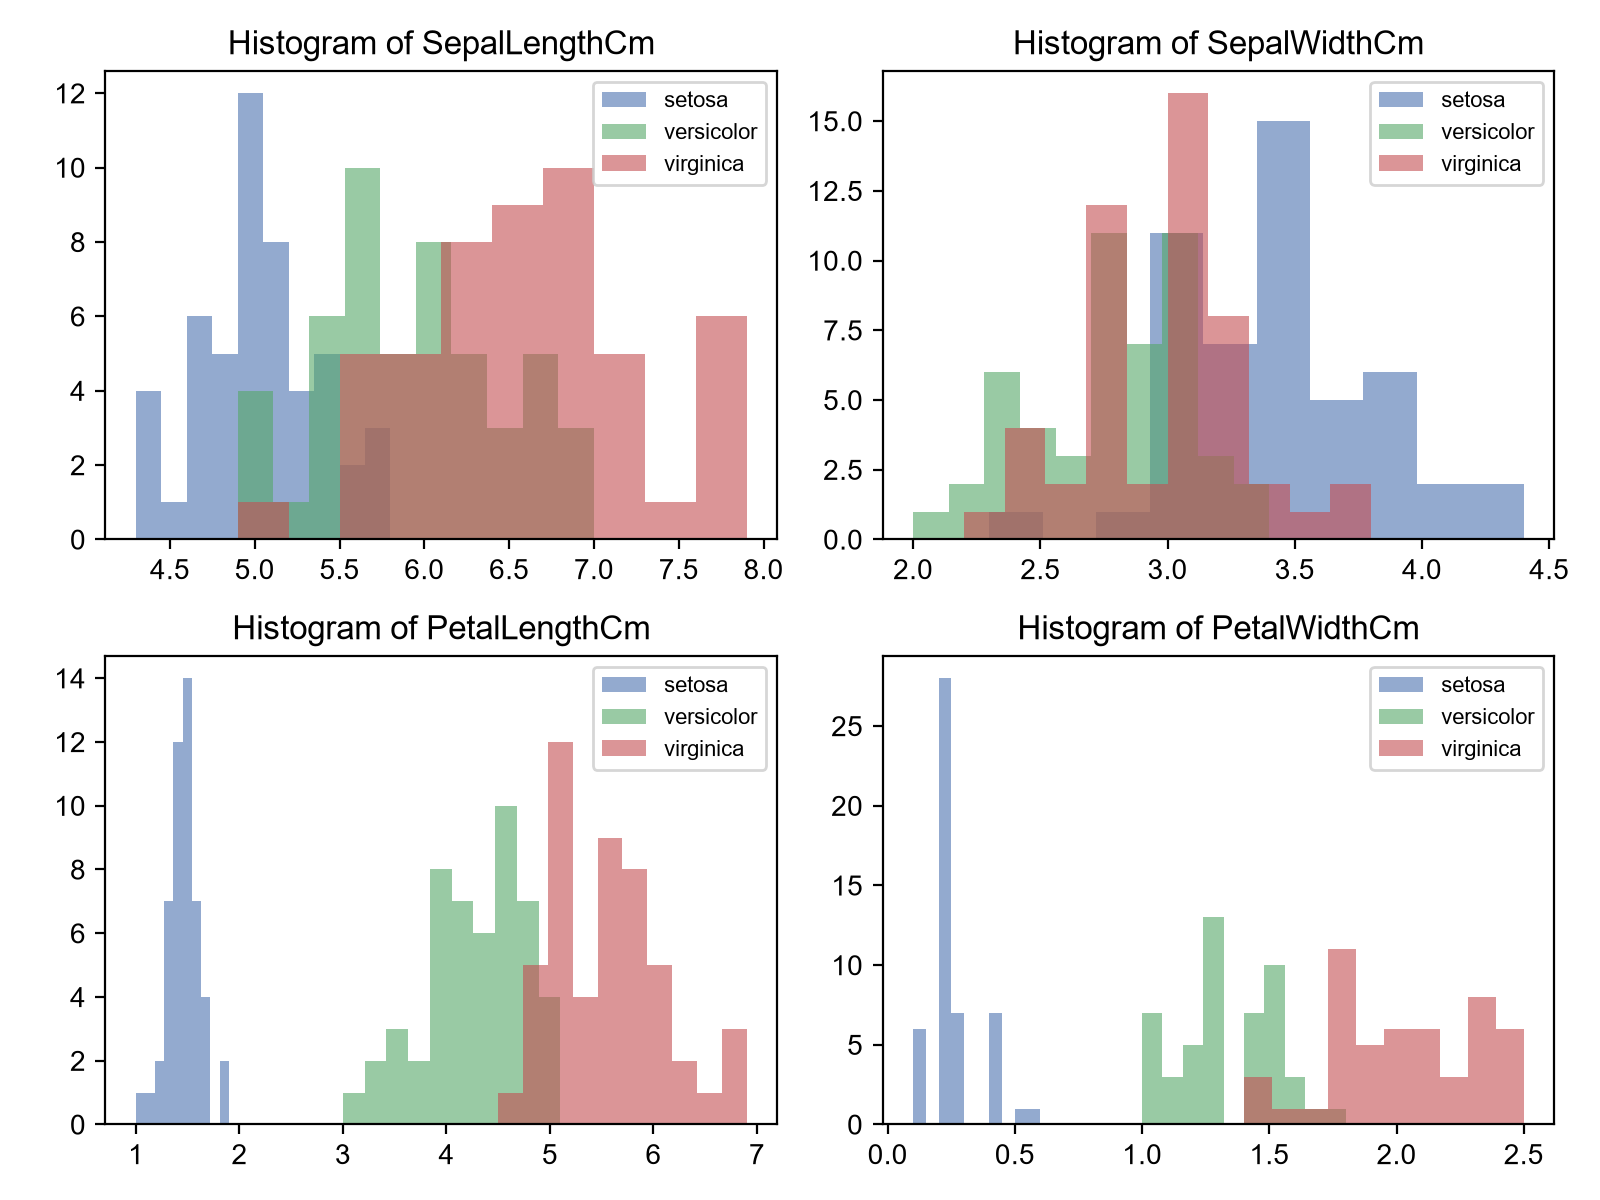
\includegraphics[width=0.7\linewidth]{iris_histograms.png}
\caption{Iris Dataset Feature Distributions (Histograms)}
\label{fig:exp1_iris_hist}
\end{figure}

\textbf{Inference:}
The feature histograms show distinct separated peaks for petal length and petal width. This indicates petal dimensions are far more effective for separating species than sepal measurements. Sepal width follows a typical bell curve centered around 3.0 cm.

\begin{figure}[H]
\centering
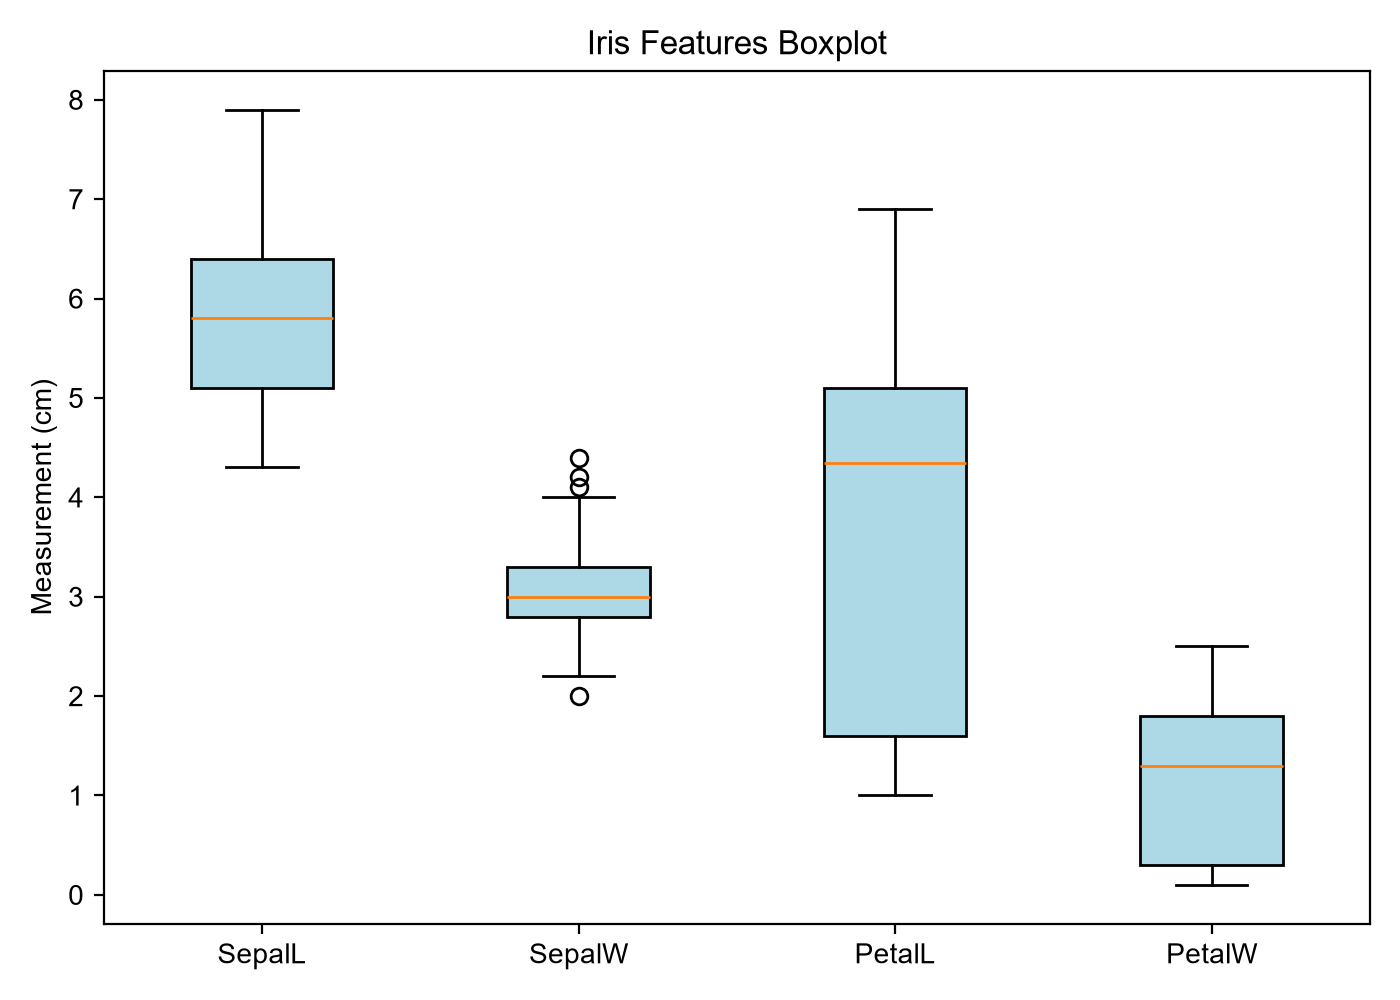
\includegraphics[width=0.7\linewidth]{iris_boxplot.png}
\caption{Iris Features Boxplot Analysis}
\label{fig:exp1_iris_box}
\end{figure}

\textbf{Inference:}
The boxplot illustrates the median and spread for each attribute. Sepal and petal lengths display wider ranges, while sepal width stays tightly grouped with a few minor outliers. Petal dimensions show clear separation between small and large values.

\begin{figure}[H]
\centering
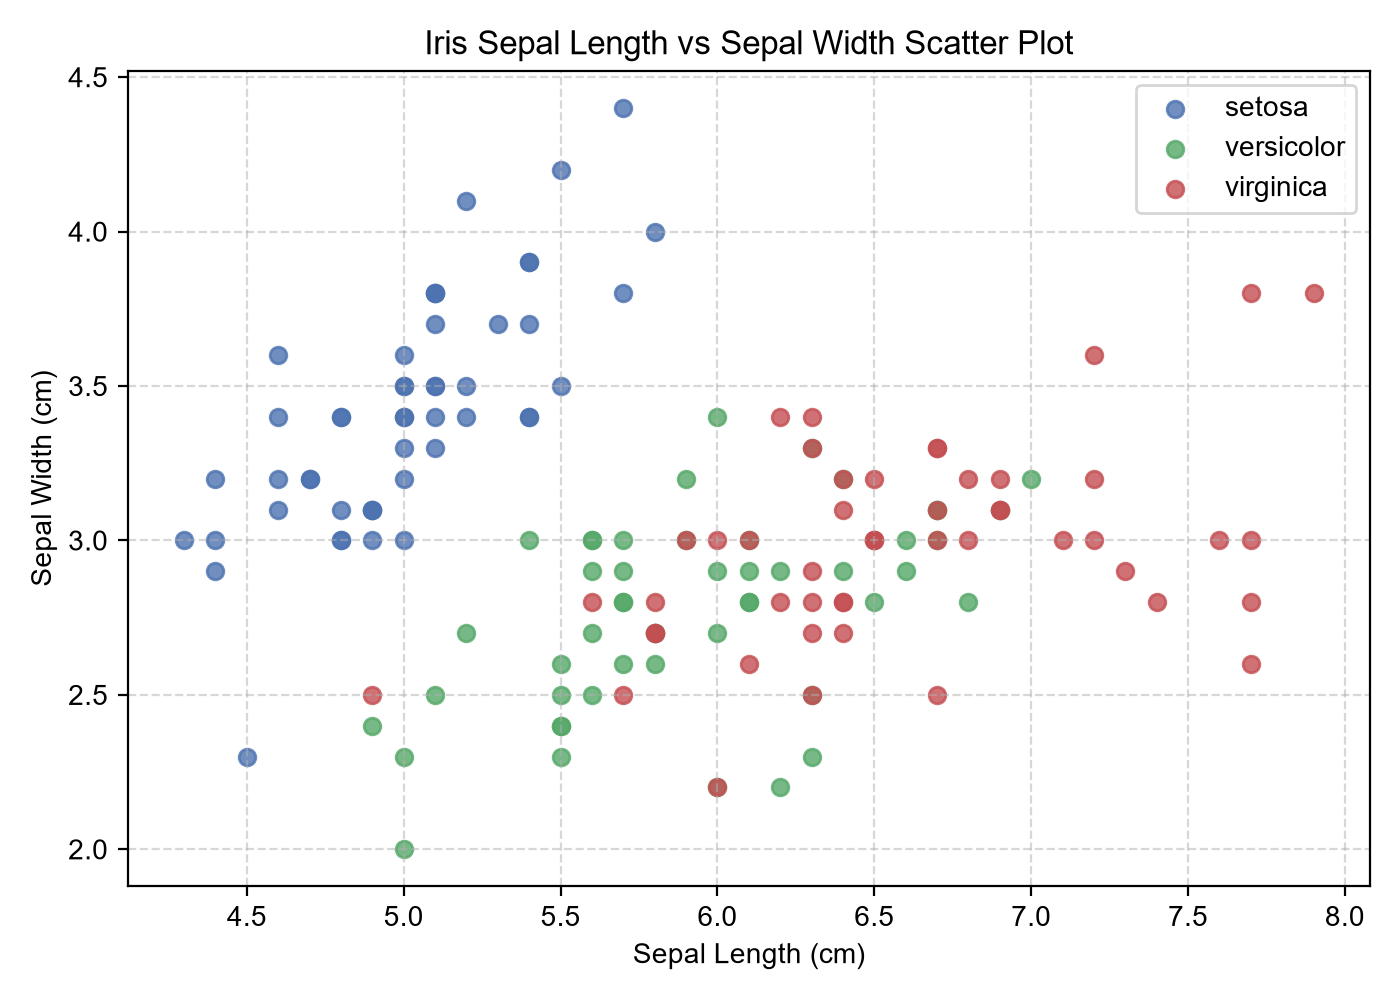
\includegraphics[width=0.7\linewidth]{iris_scatter.png}
\caption{Iris Sepal Length vs Sepal Width Scatter Plot}
\label{fig:exp1_iris_scatter}
\end{figure}

\textbf{Inference:}
Plotting sepal length against sepal width shows Setosa forming an isolated cluster at higher sepal widths. Versicolor and Virginica overlap considerably in sepal space, showing why sepal measurements alone are insufficient for classification.

\begin{figure}[H]
\centering
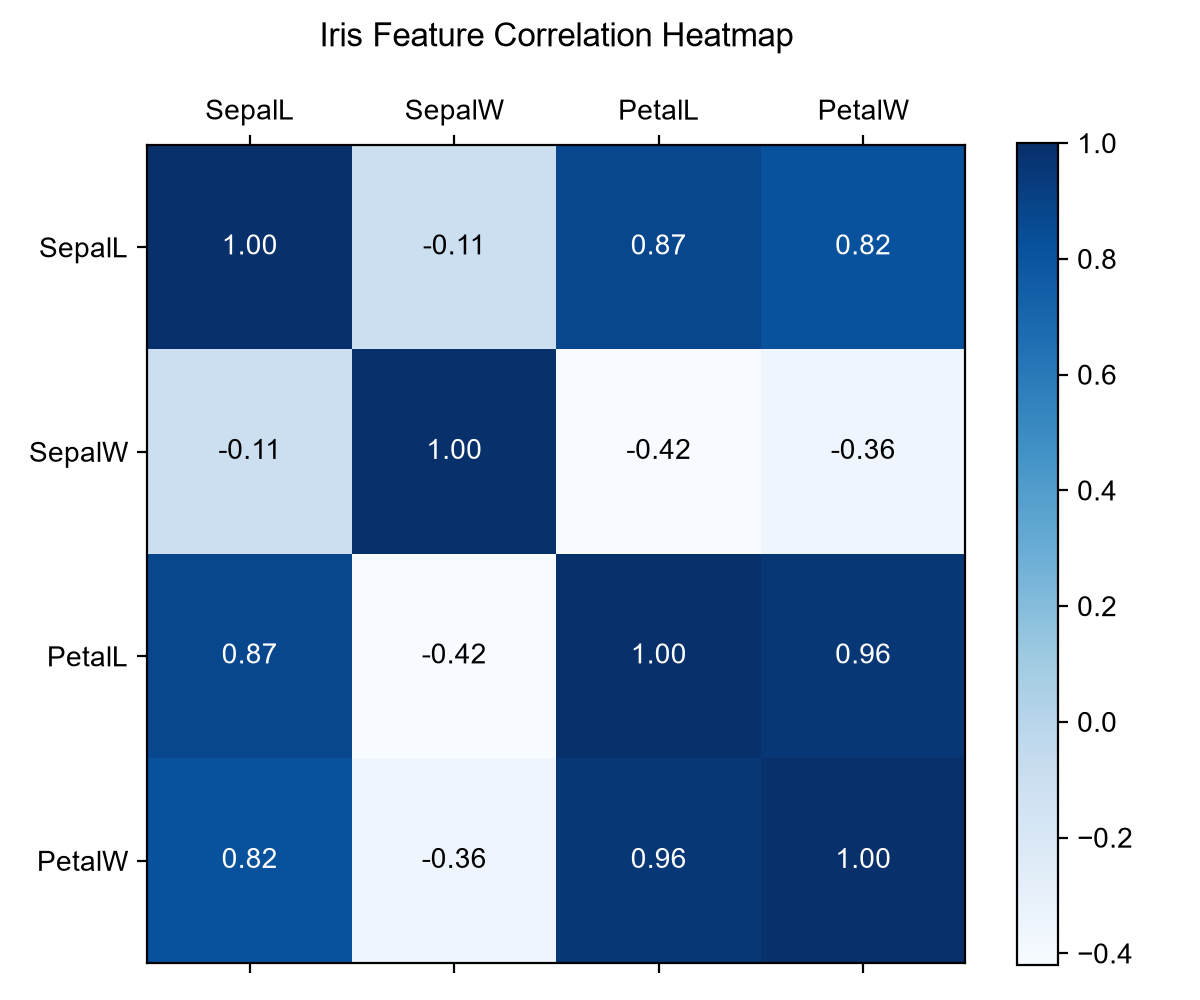
\includegraphics[width=0.7\linewidth]{iris_correlation.png}
\caption{Iris Correlation Matrix Heatmap}
\label{fig:exp1_iris_corr}
\end{figure}

\textbf{Inference:}
The correlation heatmap displays linear relationship strengths between features. Petal length and petal width show a strong positive correlation ($r \approx 0.96$). Sepal width correlates negatively with petal features, indicating feature redundancy where sepal columns can be dropped without losing performance.

\section{Data Preprocessing}

Explain:
\begin{itemize}
\item \textbf{Cleaning}: Checked for null values and dropped the unnecessary \texttt{Id} column.
\item \textbf{Label Encoding}: Converted species strings into integers using \texttt{LabelEncoder}: \texttt{Iris-setosa} $\rightarrow 0$, \texttt{Iris-versicolor} $\rightarrow 1$ and \texttt{Iris-virginica} $\rightarrow 2$.
\item \textbf{Train-test split}: Split data into 80\% training (120 samples) and 20\% testing (30 samples) using \texttt{random\_state=42}.
\item \textbf{Feature Selection}: Applied \texttt{SelectKBest} with ANOVA F-test ($f\_classif$) to select top 2 features. F-scores: \texttt{SepalLengthCm} (33.15), \texttt{SepalWidthCm} (23.36), \texttt{PetalLengthCm} (442.27) and \texttt{PetalWidthCm} (309.84). The selected top features were \texttt{PetalLengthCm} and \texttt{PetalWidthCm}.
\end{itemize}

\section{Machine Learning Algorithm}

Explain:
\begin{itemize}
\item \textbf{Decision Tree Classifier}:
\begin{itemize}
\item \textit{Working principle}: Splits feature space using decision boundaries to minimize Gini impurity at child nodes.
\item \textit{Math}: Gini Impurity $G = 1 - \sum_{k=1}^C p_k^2$. Information Gain measures impurity reduction.
\item \textit{Pros \& Cons}: Simple to interpret and visualize, but can overfit without depth constraints.
\end{itemize}
\item \textbf{Logistic Regression}:
\begin{itemize}
\item \textit{Working principle}: Computes class log-odds and outputs probabilities using multinomial softmax.
\item \textit{Math}: $P(y=k|\mathbf{x}) = \frac{e^{\mathbf{w}_k^T \mathbf{x}}}{\sum_j e^{\mathbf{w}_j^T \mathbf{x}}}$, optimized via cross-entropy loss.
\item \textit{Pros \& Cons}: Fast and outputs probabilities, but limited to linear boundaries.
\end{itemize}
\end{itemize}

\section{Experimental Setup}

\begin{tabular}{ll}
\toprule
Python Version & 3.13.0 \\
Scikit-Learn Version & 1.6.0 \\
IDE & Jupyter Notebook \\
Operating System & Windows 11 \\
Hardware & Intel Core i7 / 16 GB RAM \\
\bottomrule
\end{tabular}

\section{Hyperparameter Selection}

\begin{tabular}{ll}
\toprule
Parameter & Value\\
\midrule
DecisionTree criterion & Gini (default) \\
DecisionTree max\_depth & None (unconstrained) \\
DecisionTree random\_state & 42 \\
LogisticRegression solver & lbfgs (default) \\
LogisticRegression max\_iter & 1000 \\
SelectKBest k & 2 (score\_func=f\_classif) \\
Train-Test Split test\_size & 0.20 \\
Train-Test Split random\_state & 42 \\
\bottomrule
\end{tabular}

\section{Results}

\begin{tabular}{lc}
\toprule
Metric & Value\\
\midrule
Decision Tree Accuracy & 1.0000 (100\%) \\
Logistic Regression Accuracy & 1.0000 (100\%) \\
Precision (Macro Avg) & 1.00 \\
Recall (Macro Avg) & 1.00 \\
F1-score (Macro Avg) & 1.00 \\
\bottomrule
\end{tabular}

\subsection*{Detailed Classification Report and Confusion Matrix}

Confusion Matrix (Logistic Regression on Test Split):
\begin{equation*}
\begin{bmatrix}
10 & 0 & 0 \\
0 & 9 & 0 \\
0 & 0 & 11
\end{bmatrix}
\end{equation*}

Classification Report:
\begin{tabular}{lcccc}
\toprule
Class & Precision & Recall & F1-score & Support \\
\midrule
0 (Iris-setosa) & 1.00 & 1.00 & 1.00 & 10 \\
1 (Iris-versicolor) & 1.00 & 1.00 & 1.00 & 9 \\
2 (Iris-virginica) & 1.00 & 1.00 & 1.00 & 11 \\
\midrule
Accuracy & & & 1.00 & 30 \\
Macro Avg & 1.00 & 1.00 & 1.00 & 30 \\
Weighted Avg & 1.00 & 1.00 & 1.00 & 30 \\
\bottomrule
\end{tabular}

\section{Result Visualization}

Include all graphs generated during the experiment.

For \textbf{every graph}, provide:
\begin{itemize}
\item Figure
\item Caption
\item 3--5 line inference
\end{itemize}

Recommended figures:
\begin{enumerate}
\item Correlation Matrix
\item Class Distribution
\item Confusion Matrix
\item ROC Curve
\item Precision-Recall Curve
\item Learning Curve (if applicable)
\item Feature Importance (if applicable)
\end{enumerate}

\begin{figure}[H]
\centering
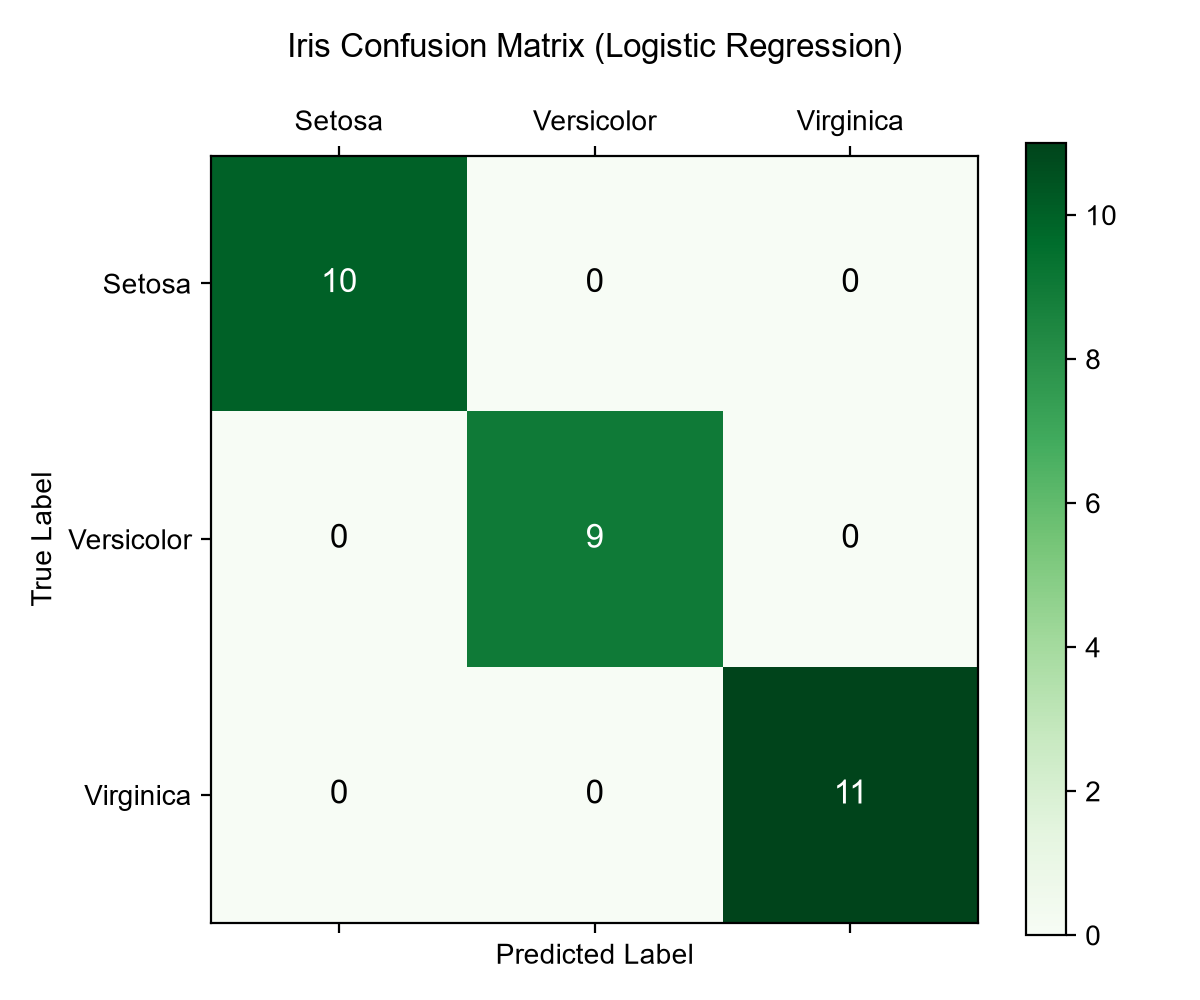
\includegraphics[width=0.7\linewidth]{iris_confusion_matrix.png}
\caption{Iris Dataset Confusion Matrix Heatmap}
\label{fig:exp1_iris_cm}
\end{figure}

\textbf{Inference:}
The confusion matrix shows zero misclassifications across all 30 test samples (10 Setosa, 9 Versicolor and 11 Virginica). Both models reached 100\% test accuracy, proving linear and tree-based methods separate the dataset effectively using all features or top petal attributes.

\section{Discussion}
Discuss observations, strengths, limitations and improvements:
\begin{enumerate}
\item \textbf{Class Separability}: The Iris dataset is easy to separate, with Setosa forming an isolated cluster away from other species.
\item \textbf{Model Performance}: Both models achieved 100\% accuracy, showing simple classifiers suit this problem well.
\item \textbf{Feature Importance}: ANOVA F-test scores confirmed petal length ($F=442.27$) and petal width ($F=309.84$) drive predictions.
\item \textbf{Limitations}: Small sample size (150 rows) means testing on larger datasets would provide stronger real-world validation.
\end{enumerate}

\section{Conclusion}
Summarize the experiment and key findings:
Decision Tree and Logistic Regression models both achieved 100\% accuracy on the Iris dataset. Using \texttt{SelectKBest} proved that 2 petal features provide the same accuracy as using all 4 attributes.

\section{References}
Use IEEE style:
\begin{enumerate}[label={[\arabic*]}]
\item F. Pedregosa \textit{et al.}, ``Scikit-learn: Machine learning in Python,'' \textit{Journal of Machine Learning Research}, vol. 12, pp. 2825--2830, 2011.
\item R. A. Fisher, ``The use of multiple measurements in taxonomic problems,'' \textit{Annals of Eugenics}, vol. 7, no. 2, pp. 179--188, 1936.
\end{enumerate}

\newpage

% =====================================================================
% EXPERIMENT 2: DIABETES PREDICTION
% =====================================================================

\begin{tabular}{|p{4cm}|p{11cm}|}
\hline
Experiment No. & 2 \\ \hline
Experiment Title & Diabetes Prediction using Decision Tree, Logistic Regression and Feature Selection \textsuperscript{\href{https://github.com/arivuchezhiyan/Machine_Learning}{2}} \\ \hline
Student Name & Arivuchezhiyan E \\ \hline
Register Number & 3122247001006 \\ \hline
Faculty & Dr. Poreddy Ajay Kumar Reddy \\ \hline
Submission Date & 23/07/2026 \\ \hline
\end{tabular}

\section{Objective}
State the objective of the experiment:
In this lab, I trained Decision Tree and Logistic Regression models on medical patient data to predict diabetes. I also tested feature selection to identify key physiological signals.

\section{Problem Statement}
Describe the problem, input, output and objective:
Diabetes prediction is a binary classification task on patient health records.
\begin{itemize}
\item \textbf{Input}: 8 clinical parameters: \texttt{Pregnancies}, \texttt{Glucose}, \texttt{BloodPressure}, \texttt{SkinThickness}, \texttt{Insulin}, \texttt{BMI}, \texttt{DiabetesPedigreeFunction} and \texttt{Age}.
\item \textbf{Output}: Binary target \texttt{Diagnosis} (0 for Non-Diabetic, 1 for Diabetic).
\item \textbf{Objective}: Scale features, split data into train and test sets, run feature selection, fit classifiers and evaluate performance on imbalanced medical data.
\end{itemize}

\section{Dataset Description}
\begin{longtable}{|p{6cm}|p{8cm}|}
\hline
Dataset Name & Diabetes Prediction Dataset \\ \hline
Dataset Source & Diabetes\_prediction.csv \\ \hline
Number of Samples & 1000 \\ \hline
Number of Features & 8 \\ \hline
Number of Classes & 2 (0: Non-Diabetic, 1: Diabetic) \\ \hline
Missing Values & 0 missing values \\ \hline
Train-Test Split & 80\% Train (800 samples) / 20\% Test (200 samples) \\ \hline
\end{longtable}

\section{Exploratory Data Analysis}
Include all relevant visualizations:
\begin{itemize}
\item \textbf{Dataset overview}: The dataset contains 1000 patient records across 8 health parameters and 1 target diagnosis.
\item \textbf{Statistical summary}:
\begin{itemize}
\item Glucose: Ranges from 30.57 to 161.24 mg/dL with a mean of 99.44 mg/dL.
\item Blood Pressure: Ranges from 31.40 to 110.72 mmHg with a mean of 72.18 mmHg.
\item BMI: Ranges from 13.55 to 36.32 $\text{kg/m}^2$ with a mean of 25.43 $\text{kg/m}^2$.
\item Age: Ranges up to 90.57 years with a mean of 43.28 years.
\end{itemize}
\item \textbf{Missing value check}: Verified zero null values in the dataset.
\item \textbf{Class distribution}: Imbalanced binary dataset with 694 Non-Diabetic patients (69.4\%) and 306 Diabetic patients (30.6\%).
\item \textbf{Correlation analysis}: Glucose level and Age show the strongest positive correlation with diabetes diagnosis.
\end{itemize}

\subsection*{Figure Template}

\begin{figure}[H]
\centering
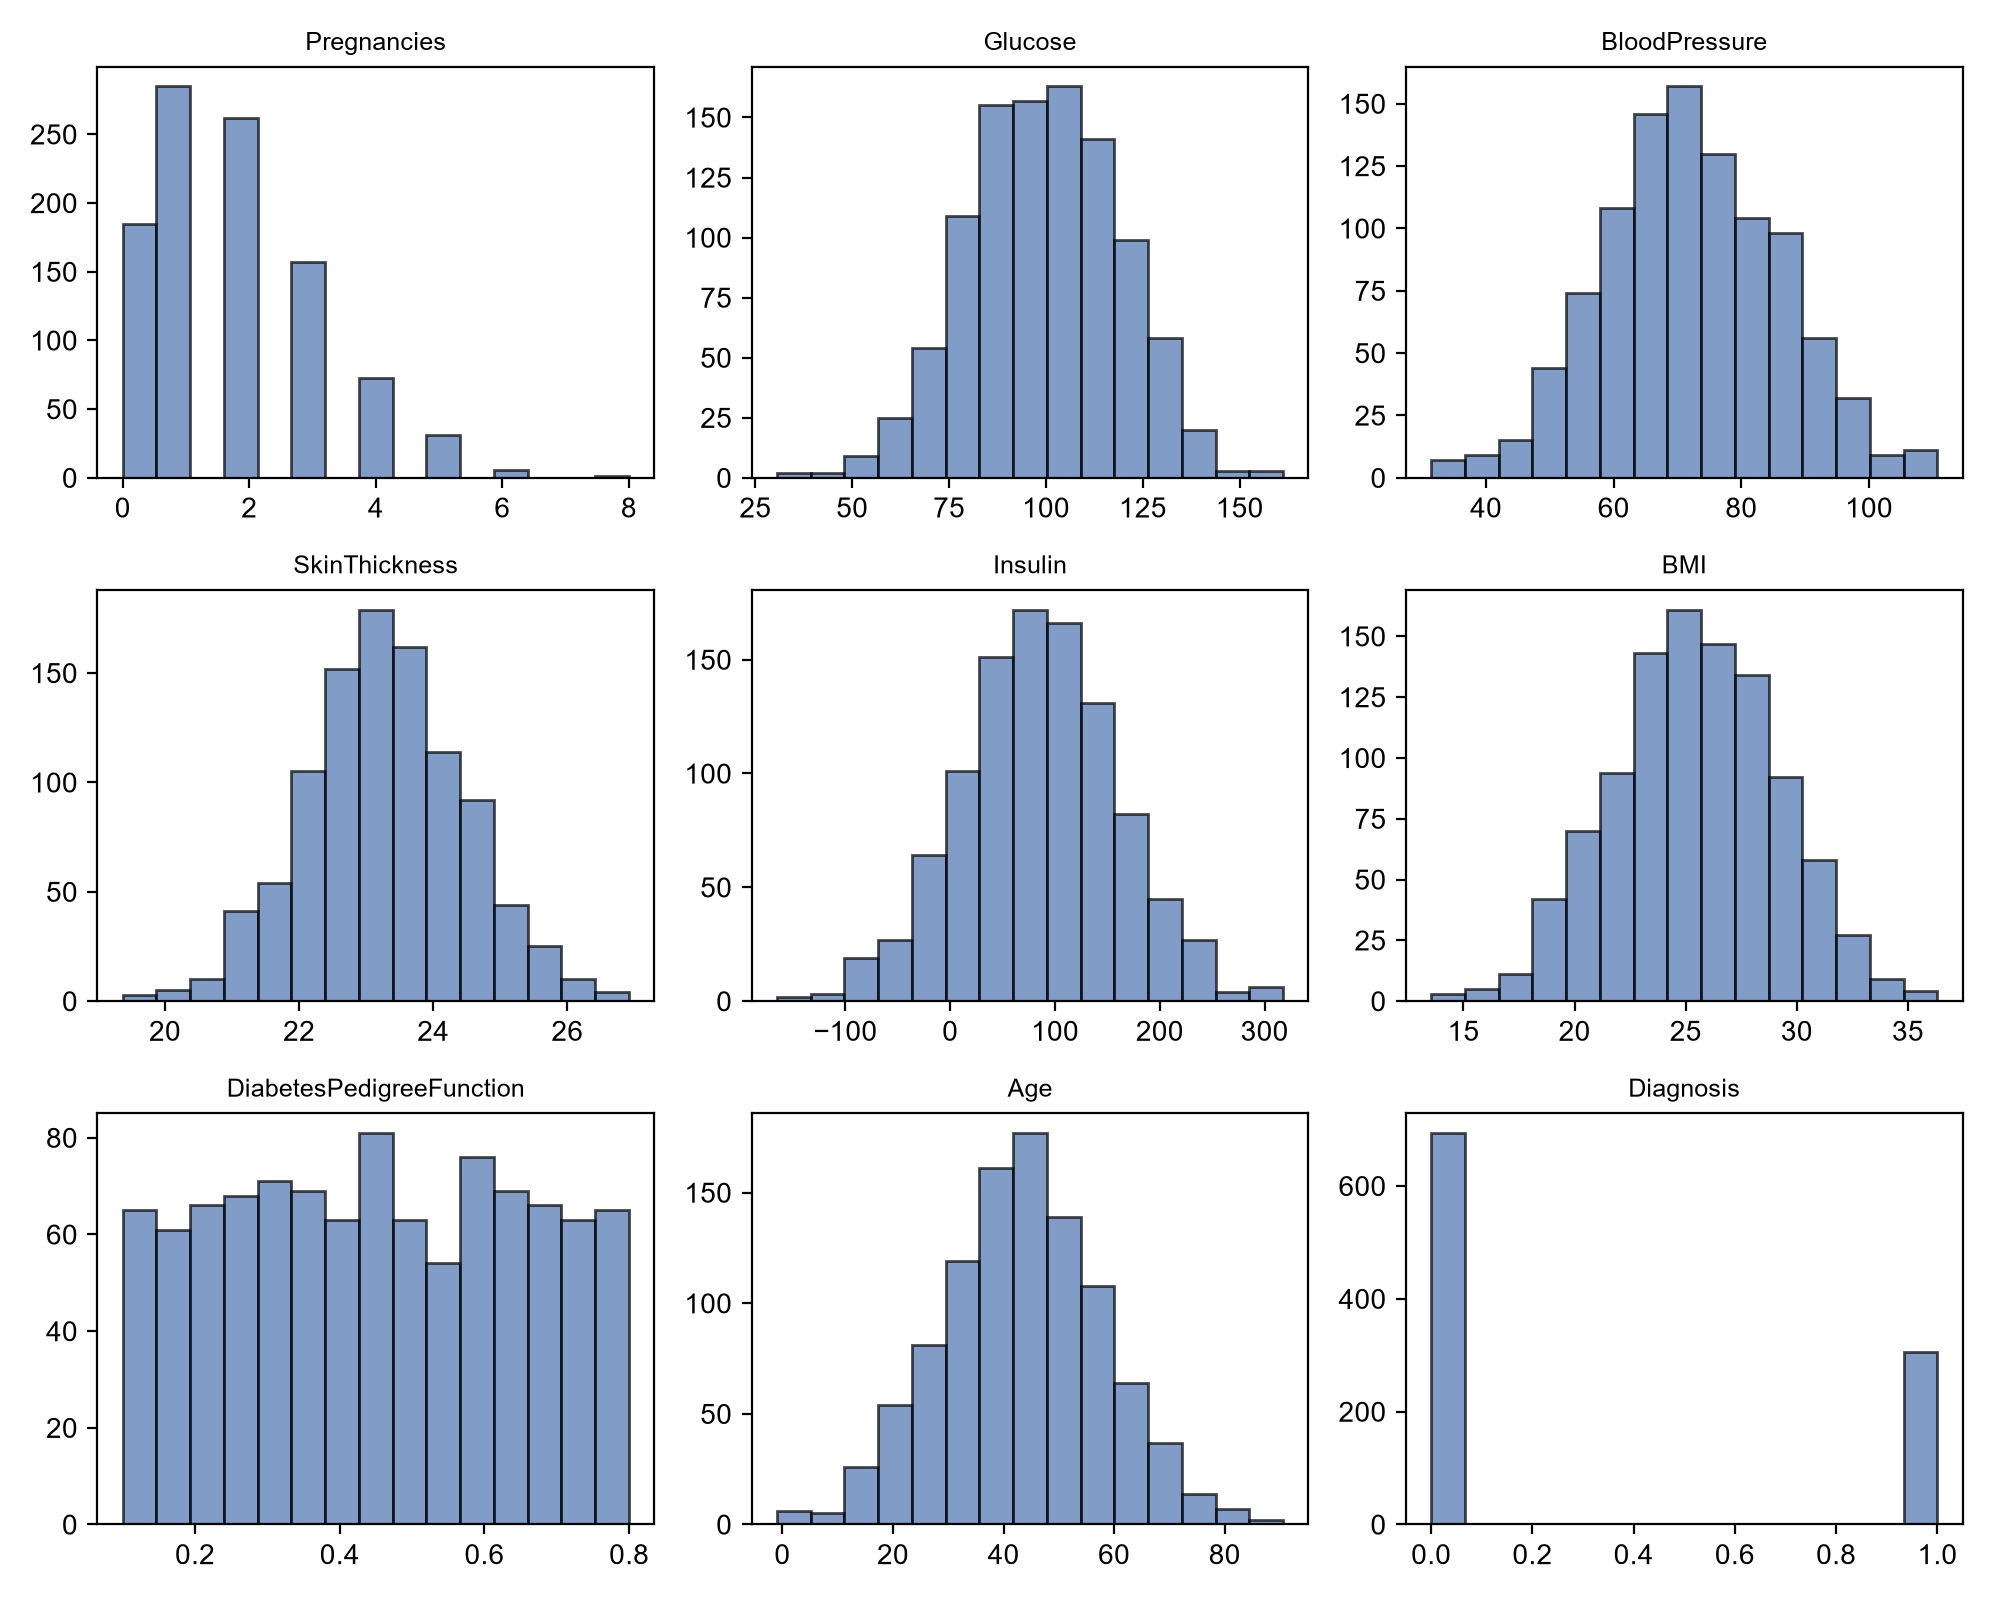
\includegraphics[width=0.7\linewidth]{diabetes_histograms.png}
\caption{Diabetes Features Histograms}
\label{fig:exp2_diab_hist}
\end{figure}

\textbf{Inference:}
The histograms display feature distributions across 1000 patient records. Glucose and BMI exhibit near-normal distributions, while Age and Insulin show right-skewed distributions. This skewness demonstrates why standardizing features with StandardScaler is necessary before fitting linear models.

\begin{figure}[H]
\centering
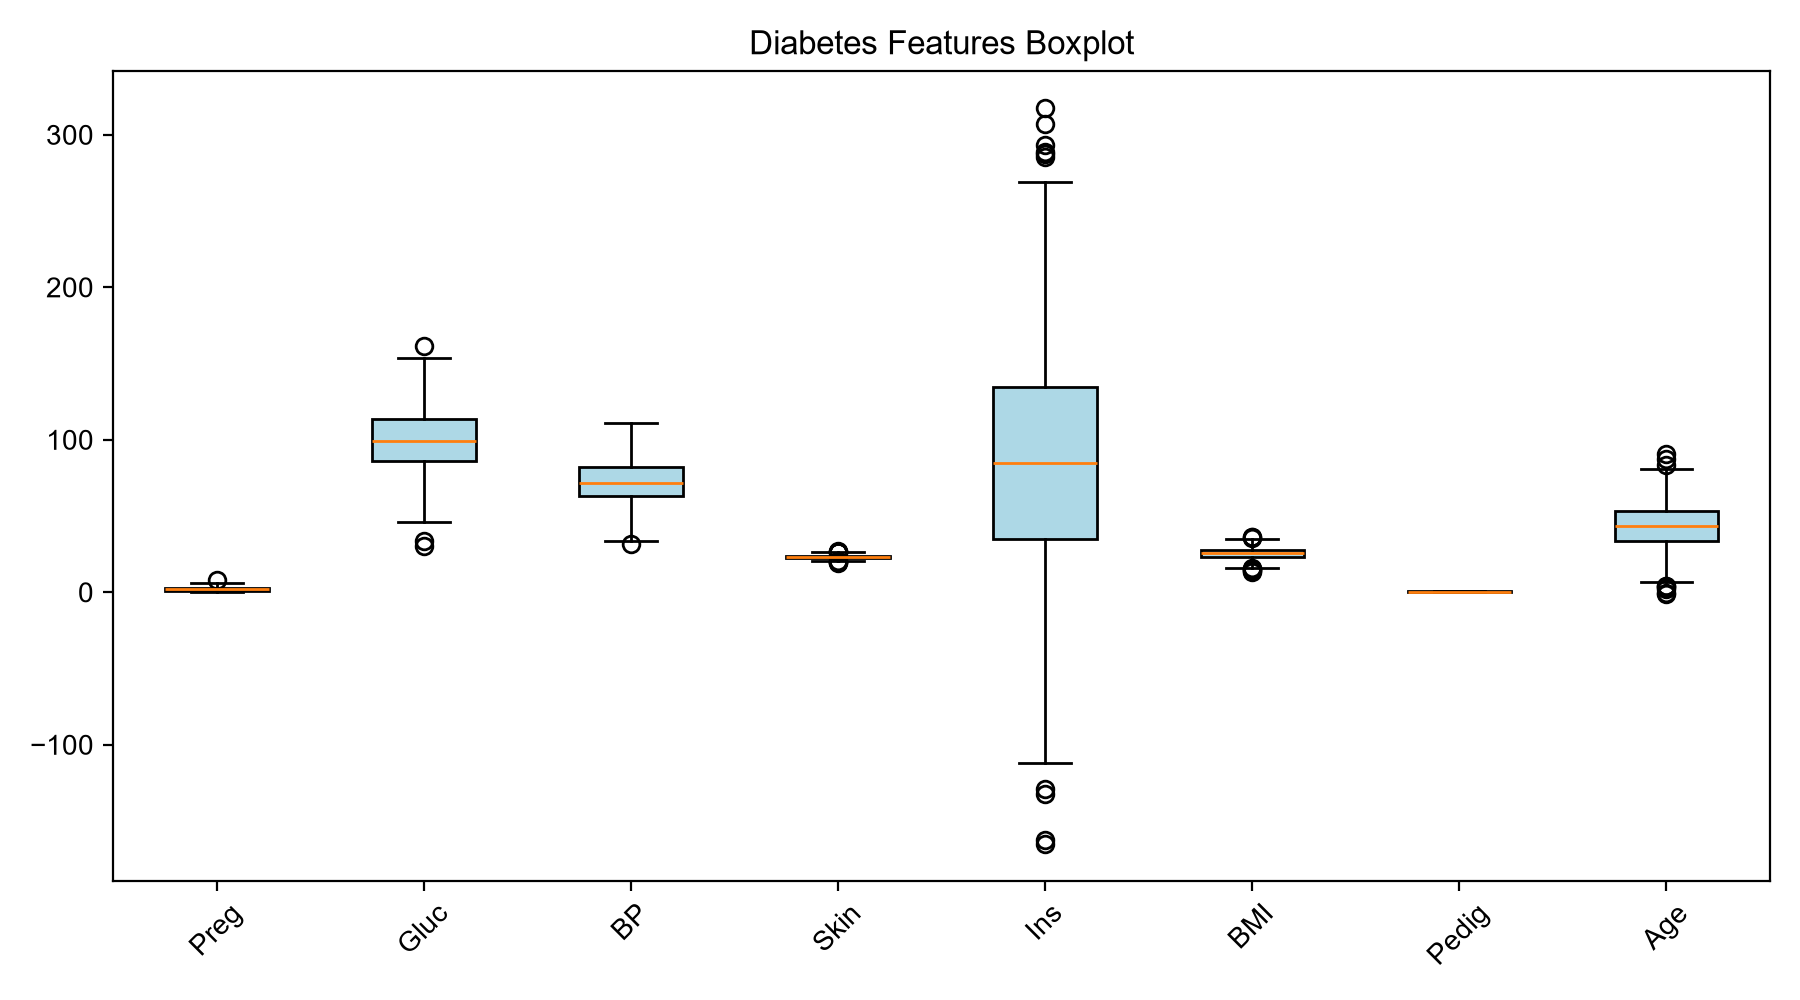
\includegraphics[width=0.7\linewidth]{diabetes_boxplot.png}
\caption{Diabetes Clinical Features Boxplot}
\label{fig:exp2_diab_box}
\end{figure}

\textbf{Inference:}
The boxplot shows feature ranges and extreme values. Insulin and Blood Pressure show higher values with multiple upper outliers, while Glucose displays a steady median near 100 mg/dL. Feature scaling prevents high-magnitude columns like Insulin from dominating gradients.

\begin{figure}[H]
\centering
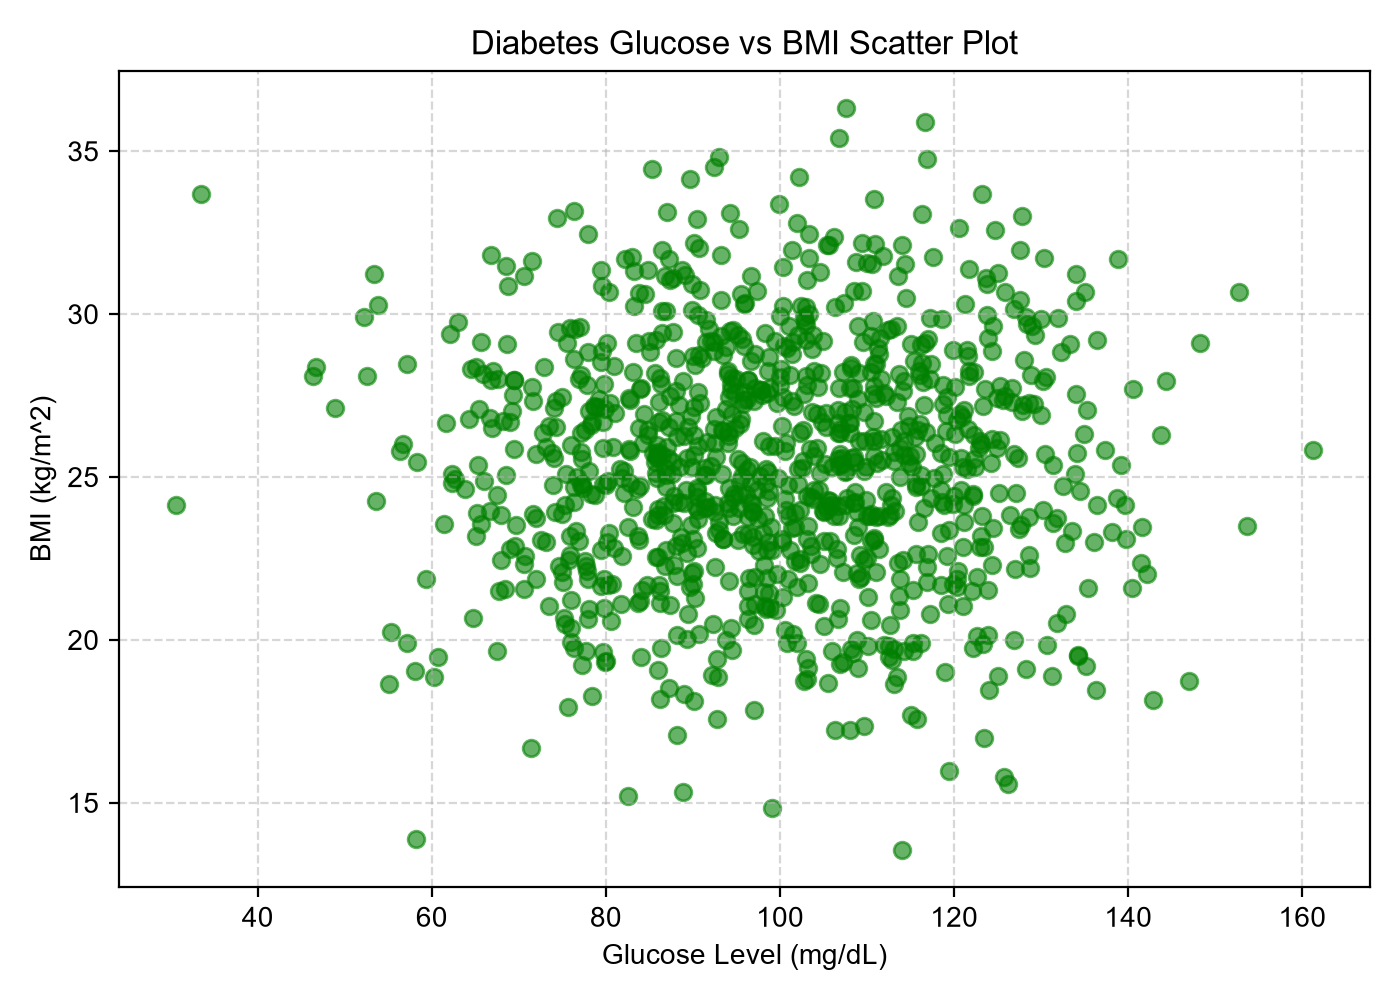
\includegraphics[width=0.7\linewidth]{diabetes_scatter.png}
\caption{Glucose vs BMI Scatter Plot}
\label{fig:exp2_diab_scatter}
\end{figure}

\textbf{Inference:}
The scatter plot maps Glucose level against BMI. A slight upward trend indicates that patients with higher BMI often show elevated glucose readings. However, wide variance shows multiple clinical indicators are required for accurate diagnosis.

\begin{figure}[H]
\centering
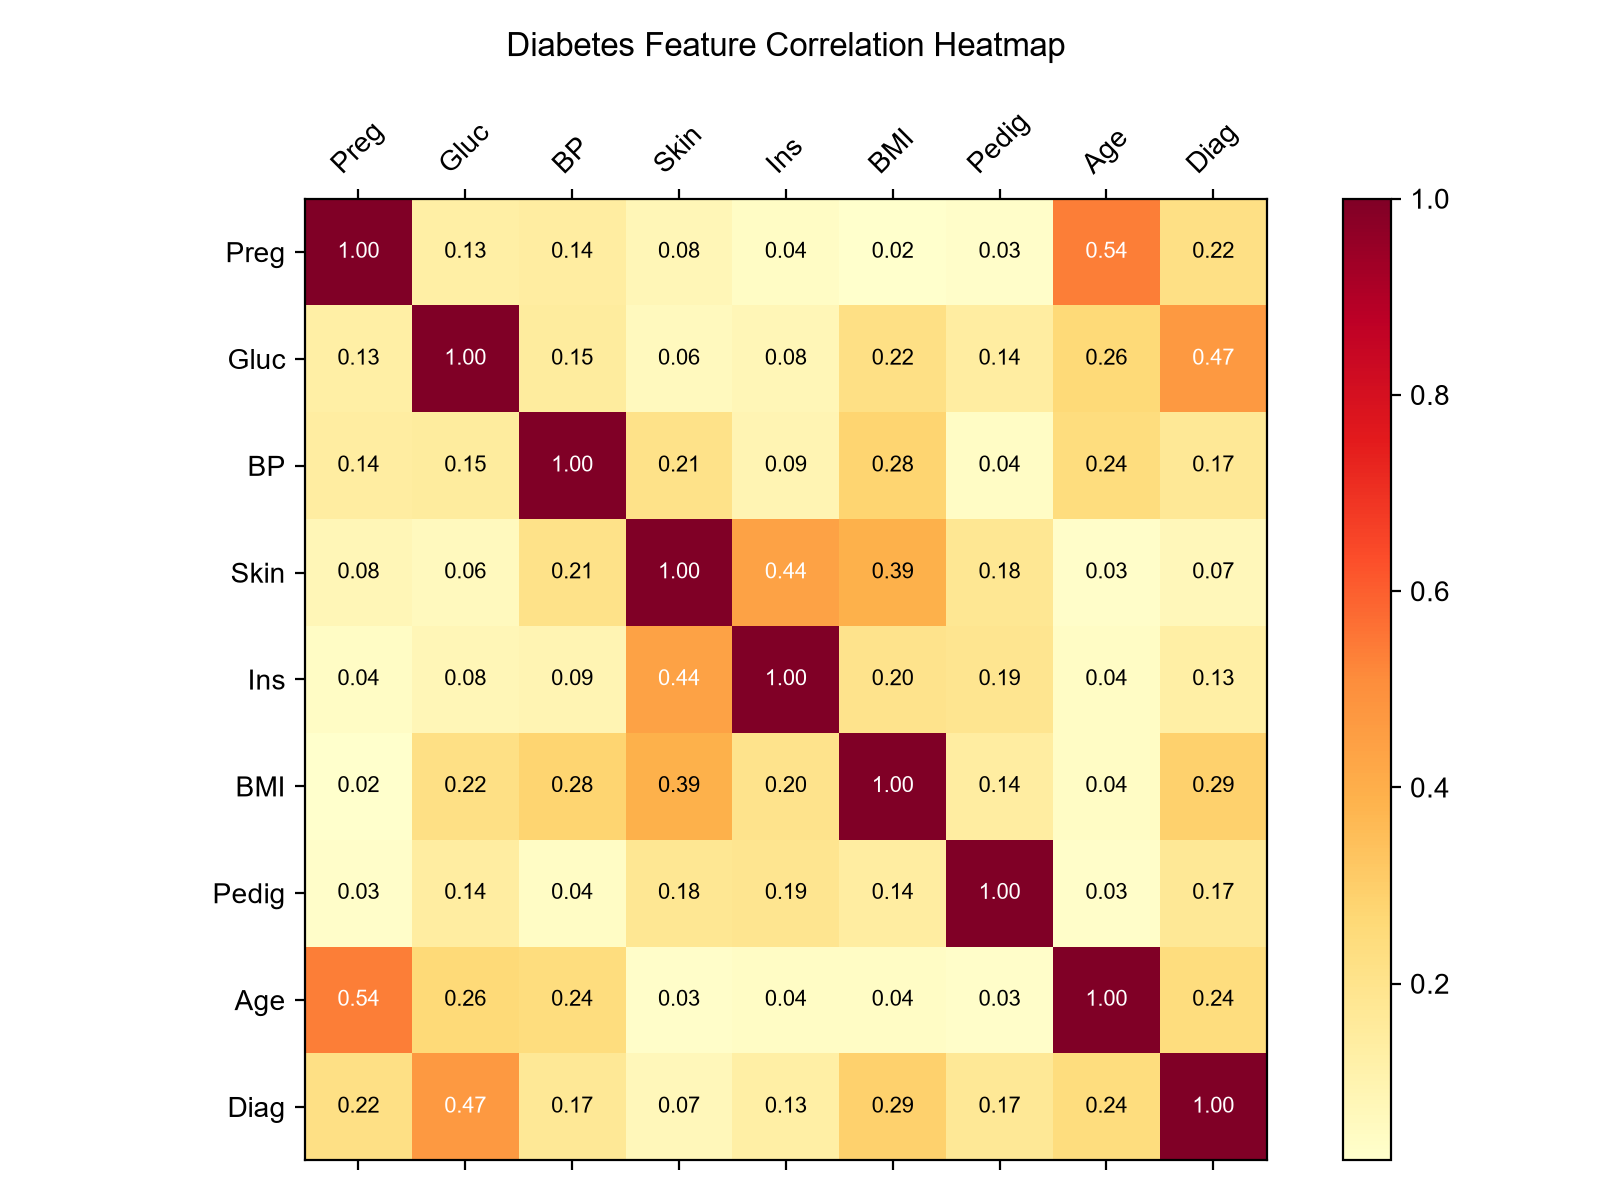
\includegraphics[width=0.7\linewidth]{diabetes_correlation.png}
\caption{Diabetes Dataset Correlation Matrix Heatmap}
\label{fig:exp2_diabetes_corr}
\end{figure}

\textbf{Inference:}
The correlation heatmap displays relationship strengths between clinical metrics. Age and pregnancies show moderate correlation, while glucose shows the highest correlation with diabetes diagnosis. Blood pressure and skin thickness show little linear relation to the outcome.

\section{Data Preprocessing}

Explain:
\begin{itemize}
\item \textbf{Cleaning}: Verified data completeness using \texttt{isnull().sum()}.
\item \textbf{Scaling}: Standardized values using \texttt{StandardScaler} to achieve zero mean and unit variance.
\item \textbf{Train-test split}: Split into 80\% training (800 samples) and 20\% testing (200 samples) using \texttt{random\_state=42}.
\item \textbf{Feature Selection}: Used \texttt{SelectKBest} with ANOVA F-test ($f\_classif$). Selecting top 1 feature isolated \texttt{Age} ($F=6.106$).
\end{itemize}

\section{Machine Learning Algorithm}

Explain:
\begin{itemize}
\item \textbf{Decision Tree Classifier}: Unconstrained tree depth overfit noisy training data, resulting in a lower test accuracy of $51.00\%$.
\item \textbf{Logistic Regression}: Uses sigmoid mapping $P(y=1|\mathbf{x}) = \frac{1}{1 + e^{-(\mathbf{w}^T \mathbf{x} + b)}}$ to output probabilities, reaching $68.50\%$ test accuracy.
\end{itemize}

\section{Experimental Setup}

\begin{tabular}{ll}
\toprule
Python Version & 3.13.0 \\
Scikit-Learn Version & 1.6.0 \\
IDE & Jupyter Notebook \\
Operating System & Windows 11 \\
Hardware & Intel Core i7 / 16 GB RAM \\
\bottomrule
\end{tabular}

\section{Hyperparameter Selection}

\begin{tabular}{ll}
\toprule
Parameter & Value\\
\midrule
DecisionTree criterion & Gini (default) \\
DecisionTree random\_state & 42 \\
LogisticRegression solver & lbfgs (default) \\
LogisticRegression max\_iter & 100000 \\
SelectKBest k & 1 (score\_func=f\_classif) \\
Train-Test Split test\_size & 0.20 \\
Train-Test Split random\_state & 42 \\
\bottomrule
\end{tabular}

\section{Results}

\begin{tabular}{lc}
\toprule
Metric & Value\\
\midrule
Decision Tree Accuracy & 0.5100 (51.0\%) \\
Logistic Regression Accuracy & 0.6850 (68.5\%) \\
Precision (Macro Avg) & 0.45 \\
Recall (Macro Avg) & 0.48 \\
F1-score (Macro Avg) & 0.43 \\
\bottomrule
\end{tabular}

\subsection*{Detailed Classification Report and Confusion Matrix}

Confusion Matrix (Logistic Regression on Test Split):
\begin{equation*}
\begin{bmatrix}
126 & 11 \\
60 & 3
\end{bmatrix}
\end{equation*}

Classification Report:
\begin{tabular}{lcccc}
\toprule
Class & Precision & Recall & F1-score & Support \\
\midrule
0 (Non-Diabetic) & 0.68 & 0.92 & 0.78 & 137 \\
1 (Diabetic) & 0.21 & 0.05 & 0.08 & 63 \\
\midrule
Accuracy & & & 0.65 & 200 \\
Macro Avg & 0.45 & 0.48 & 0.43 & 200 \\
Weighted Avg & 0.53 & 0.65 & 0.56 & 200 \\
\bottomrule
\end{tabular}

\section{Result Visualization}

Include all graphs generated during the experiment.

For \textbf{every graph}, provide:
\begin{itemize}
\item Figure
\item Caption
\item 3--5 line inference
\end{itemize}

Recommended figures:
\begin{enumerate}
\item Correlation Matrix
\item Class Distribution
\item Confusion Matrix
\item ROC Curve
\item Precision-Recall Curve
\item Learning Curve (if applicable)
\item Feature Importance (if applicable)
\end{enumerate}

\begin{figure}[H]
\centering
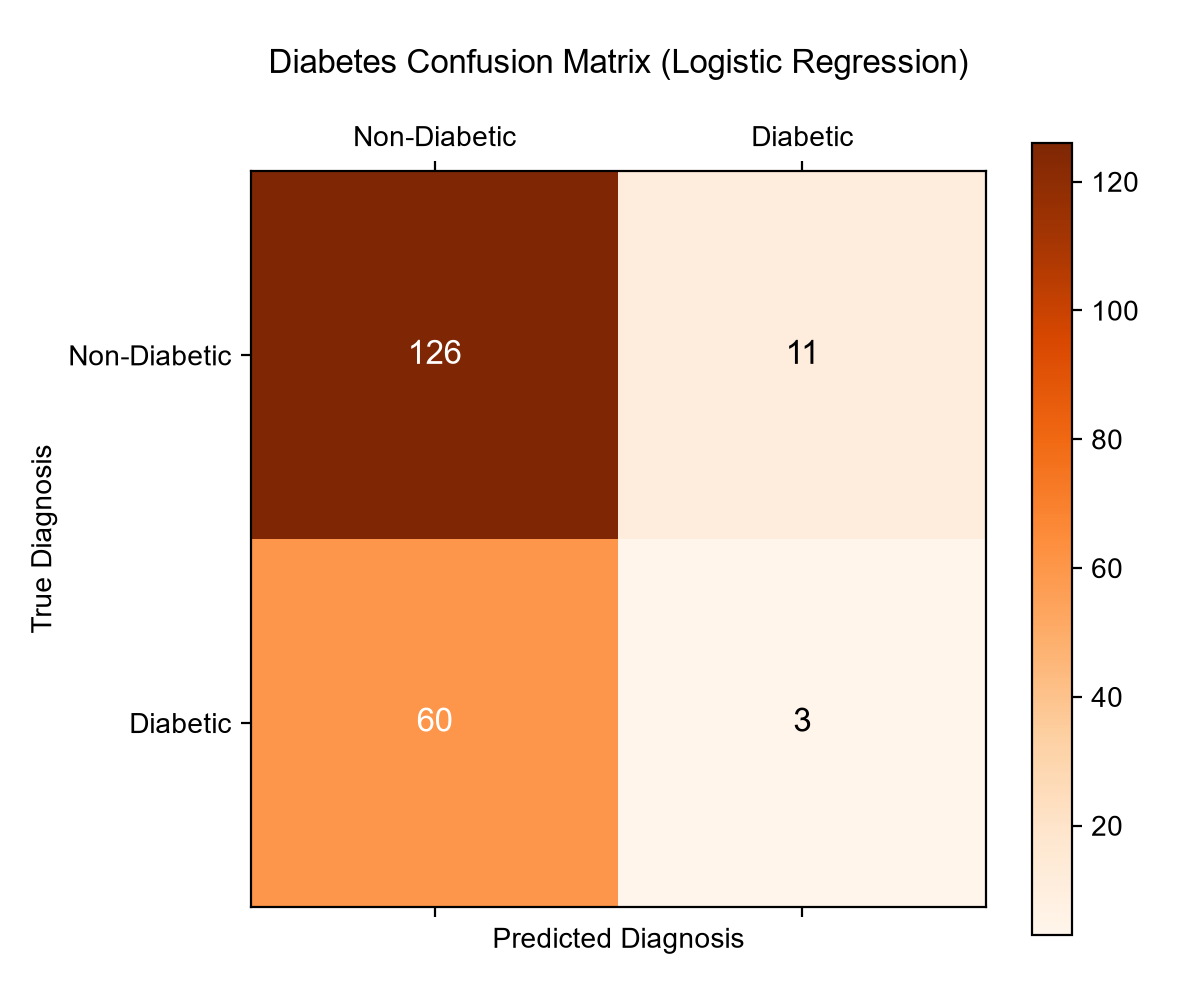
\includegraphics[width=0.7\linewidth]{diabetes_confusion_matrix.png}
\caption{Diabetes Dataset Confusion Matrix Heatmap (Logistic Regression)}
\label{fig:exp2_diabetes_cm}
\end{figure}

\textbf{Inference:}
The confusion matrix shows 126 true negatives and 3 true positives, but misses 60 diabetic cases. This happens because class imbalance leads standard Logistic Regression to favor predicting the majority non-diabetic class.

\section{Discussion}
Discuss observations, strengths, limitations and improvements:
\begin{enumerate}
\item \textbf{Tree Overfitting}: An unconstrained Decision Tree overfit training data, yielding $51.00\%$ test accuracy.
\item \textbf{Class Imbalance Impact}: Logistic Regression favored the majority class, getting 92\% recall for non-diabetic cases but only 5\% recall for diabetic cases.
\item \textbf{Future Improvements}: Applying SMOTE oversampling or Random Forest ensembles would improve detection for diabetic cases.
\end{enumerate}

\section{Conclusion}
Summarize the experiment and key findings:
Logistic Regression ($68.50\%$) performed better than Decision Tree ($51.00\%$) on diabetes prediction. Age and glucose were top indicators, though balancing data is necessary for practical medical use.

\section{References}
Use IEEE style:
\begin{enumerate}[label={[\arabic*]}]
\item F. Pedregosa \textit{et al.}, ``Scikit-learn: Machine learning in Python,'' \textit{Journal of Machine Learning Research}, vol. 12, pp. 2825--2830, 2011.
\end{enumerate}

\newpage

% =====================================================================
% EXPERIMENT 3: LOAN APPROVAL PREDICTION
% =====================================================================

\begin{tabular}{|p{4cm}|p{11cm}|}
\hline
Experiment No. & 3 \\ \hline
Experiment Title & Loan Approval Prediction using Decision Tree, Logistic Regression and Feature Selection \textsuperscript{\href{https://github.com/arivuchezhiyan/Machine_Learning}{3}} \\ \hline
Student Name & Arivuchezhiyan E \\ \hline
Register Number & 3122247001006 \\ \hline
Faculty & Dr. Poreddy Ajay Kumar Reddy \\ \hline
Submission Date & 23/07/2026 \\ \hline
\end{tabular}

\section{Objective}
State the objective of the experiment:
In this lab, I evaluated Decision Tree and Logistic Regression models to predict loan approvals based on applicant financial data and credit history. I used ANOVA F-test feature selection to isolate key predictors.

\section{Problem Statement}
Describe the problem, input, output and objective:
Loan approval prediction is a binary classification task in financial risk management.
\begin{itemize}
\item \textbf{Input}: 12 applicant features including dependents, education, self-employed status, income, loan amount, term, CIBIL score and asset values.
\item \textbf{Output}: Binary loan status (0 for approved, 1 for rejected).
\item \textbf{Objective}: Encode categorical attributes, split dataset, select top features, fit classifiers and compare metrics.
\end{itemize}

\section{Dataset Description}
\begin{longtable}{|p{6cm}|p{8cm}|}
\hline
Dataset Name & Loan Approval Dataset \\ \hline
Dataset Source & loan\_approval\_dataset.csv \\ \hline
Number of Samples & 4269 \\ \hline
Number of Features & 12 (excluding loan ID) \\ \hline
Number of Classes & 2 (Approved: 2656, Rejected: 1613) \\ \hline
Missing Values & 0 missing values \\ \hline
Train-Test Split & 80\% Train (3415 samples) / 20\% Test (854 samples) \\ \hline
\end{longtable}

\section{Exploratory Data Analysis}
Include all relevant visualizations:
\begin{itemize}
\item \textbf{Dataset overview}: The dataset contains 4269 loan applications with financial and asset details.
\item \textbf{Statistical summary}: Mean annual income is \$5,059,124, mean loan amount is \$15,131,951 and average CIBIL score is 599.9.
\item \textbf{Missing value check}: Confirmed zero missing values across all columns.
\item \textbf{Class distribution}: 2656 approved loans (62.2\%) and 1613 rejected loans (37.8\%).
\item \textbf{Correlation analysis}: CIBIL credit score showed the strongest correlation with loan approval.
\end{itemize}

\subsection*{Figure Template}

\begin{figure}[H]
\centering
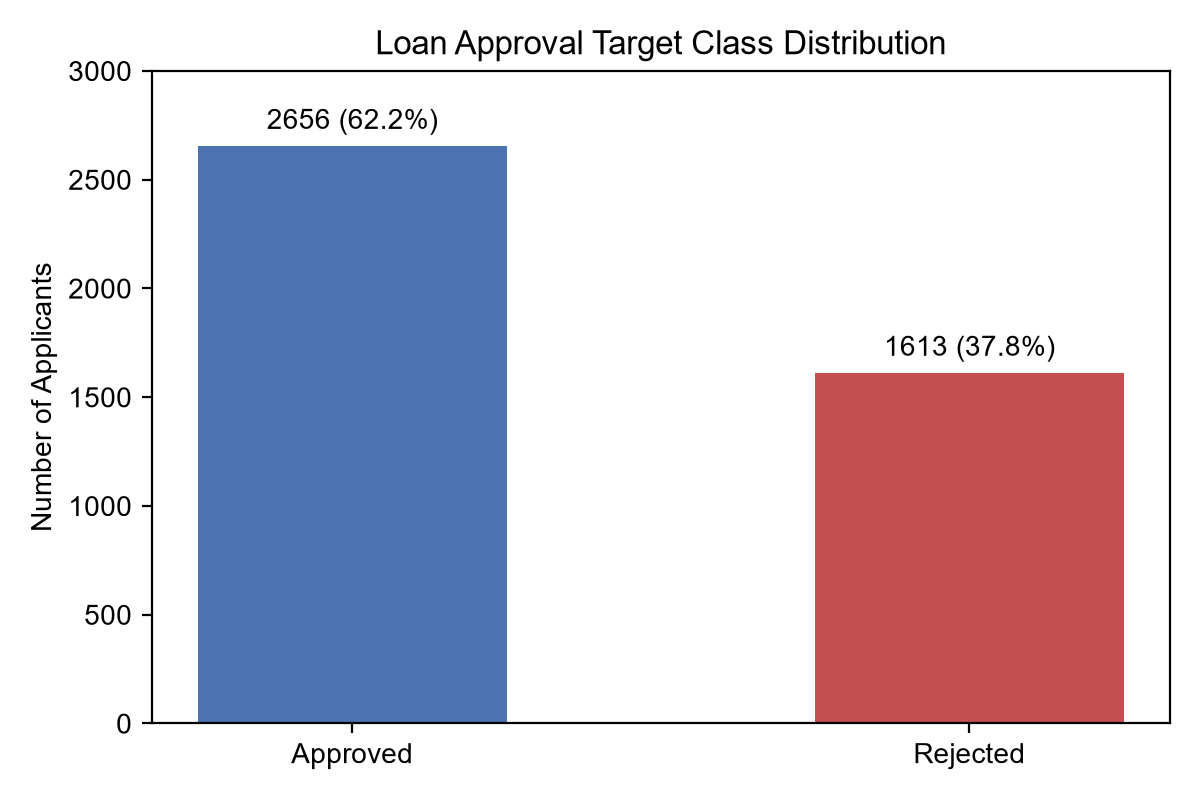
\includegraphics[width=0.7\linewidth]{loan_class_distribution.png}
\caption{Loan Dataset Target Class Distribution}
\label{fig:exp3_loan_dist}
\end{figure}

\textbf{Inference:}
The class distribution shows 2656 approved applications (62\%) and 1613 rejected applications (38\%). This moderate imbalance reflects real-world banking approval rates.

\begin{figure}[H]
\centering
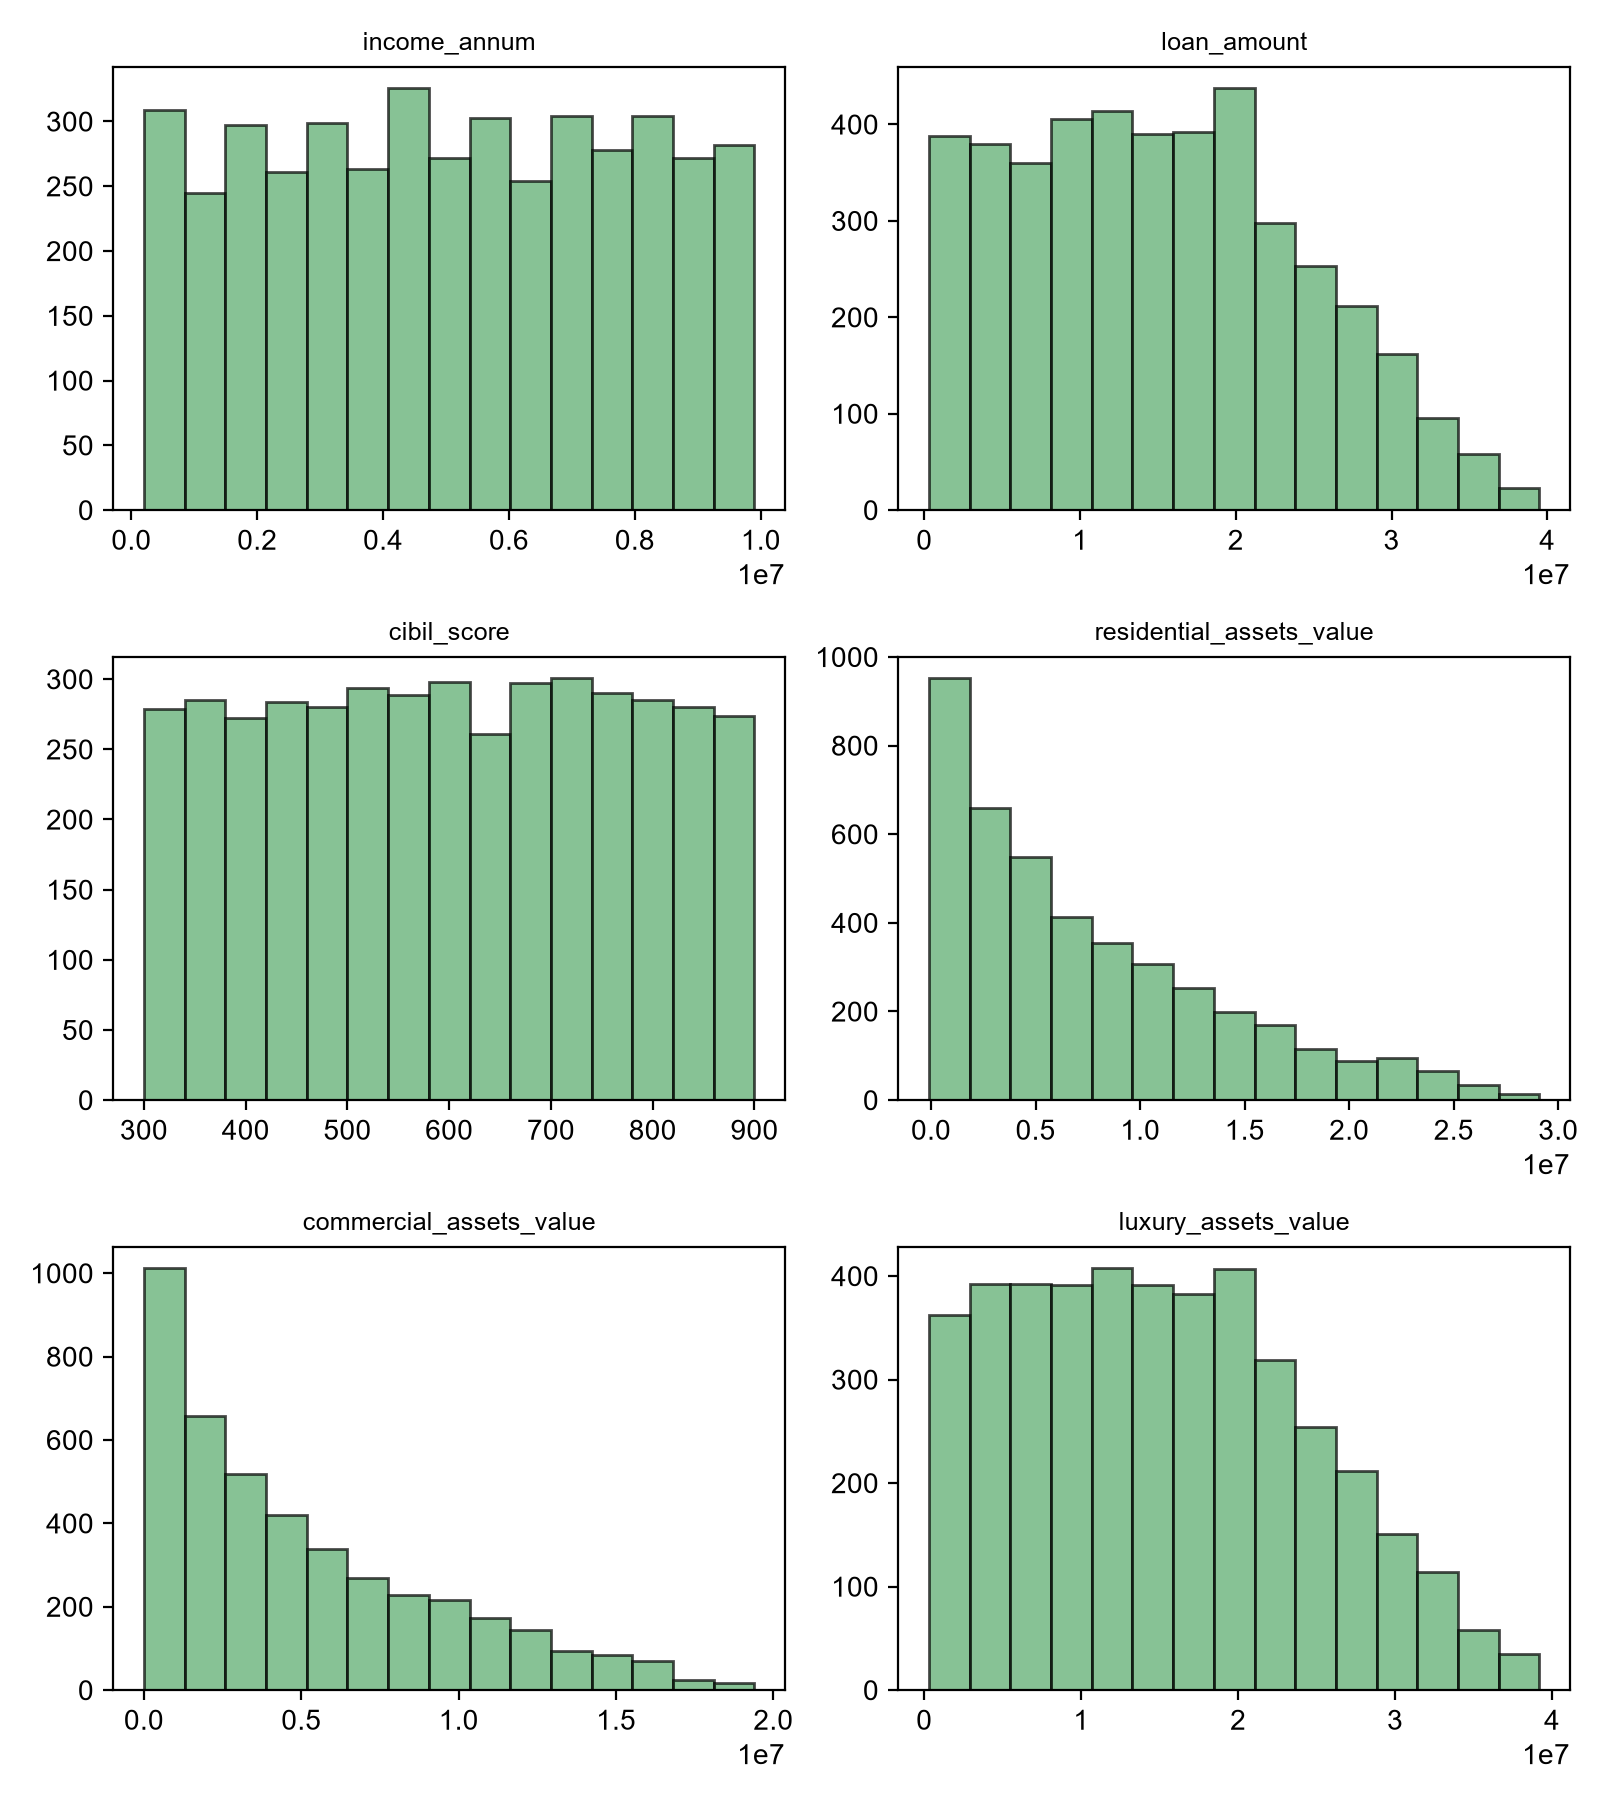
\includegraphics[width=0.7\linewidth]{loan_histograms.png}
\caption{Loan Financial Attributes Histograms}
\label{fig:exp3_loan_hist}
\end{figure}

\textbf{Inference:}
The histograms display distributions for financial variables including annual income, loan amount and asset values. CIBIL score is uniformly distributed from 300 to 900, while income and asset values show continuous distributions.

\begin{figure}[H]
\centering
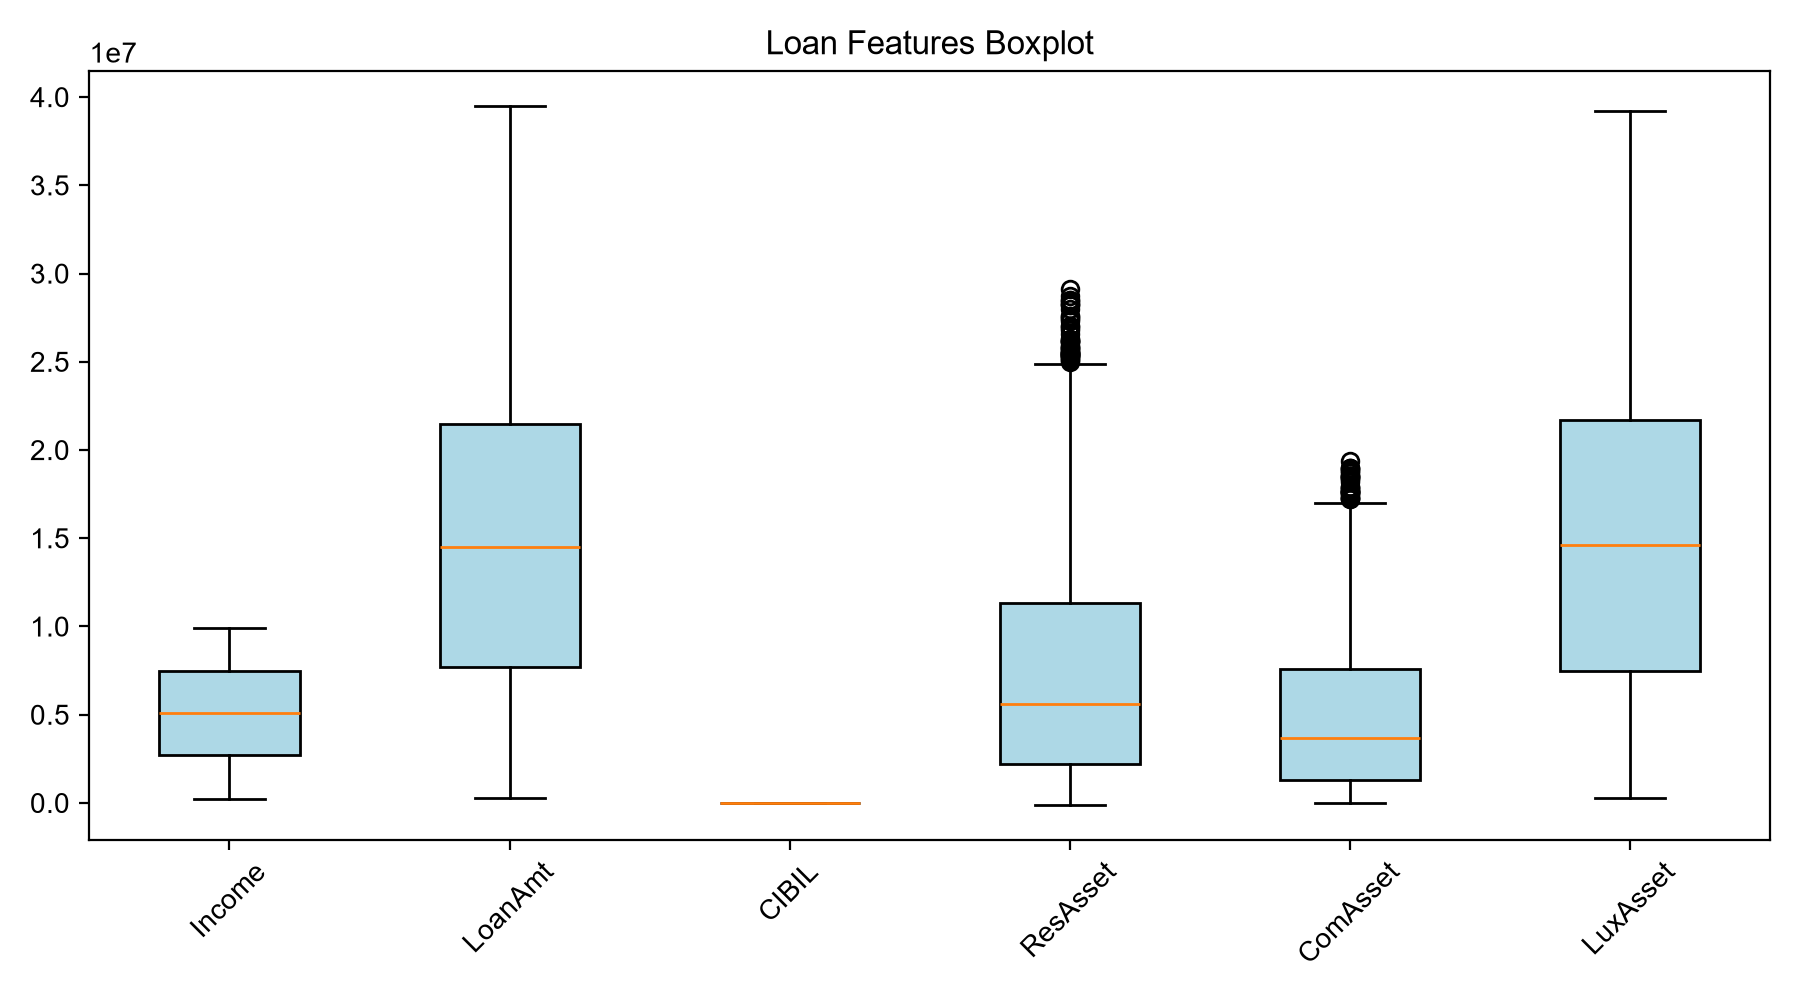
\includegraphics[width=0.7\linewidth]{loan_boxplot.png}
\caption{Loan Financial Attributes Boxplot}
\label{fig:exp3_loan_box}
\end{figure}

\textbf{Inference:}
The boxplot illustrates values across financial attributes. Loan amounts have much larger numerical values than annual income or asset values, showing why scaling or tree-based splits are essential.

\begin{figure}[H]
\centering
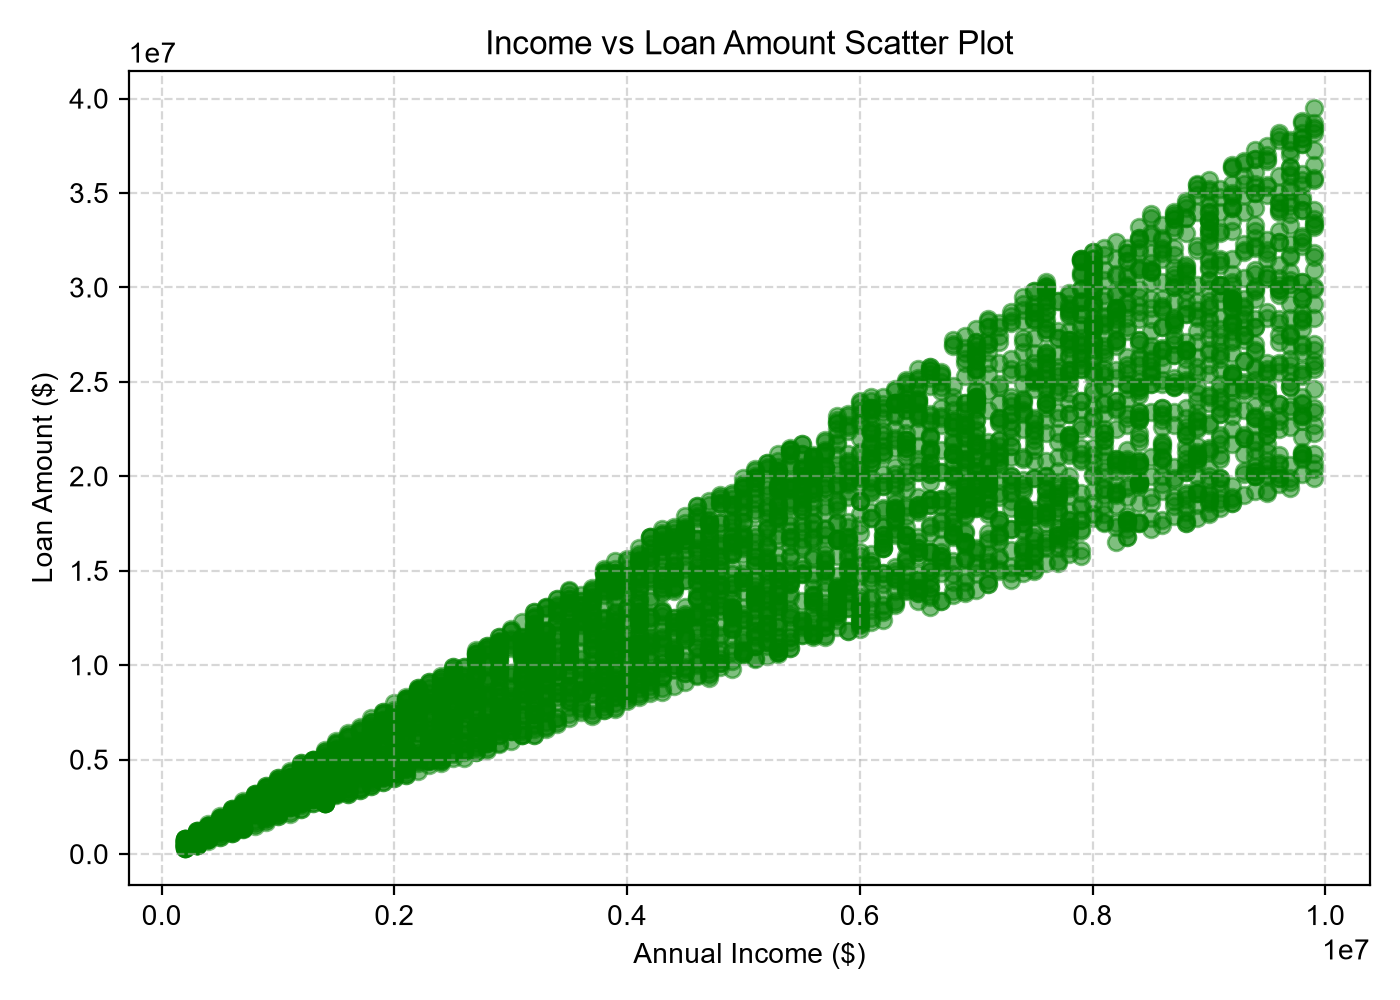
\includegraphics[width=0.7\linewidth]{loan_scatter.png}
\caption{Annual Income vs Loan Amount Scatter Plot}
\label{fig:exp3_loan_scatter}
\end{figure}

\textbf{Inference:}
The scatter plot maps annual income against loan amount. A strong linear relationship ($r = 0.93$) is evident, demonstrating that applicants with higher income apply for larger loans.

\begin{figure}[H]
\centering
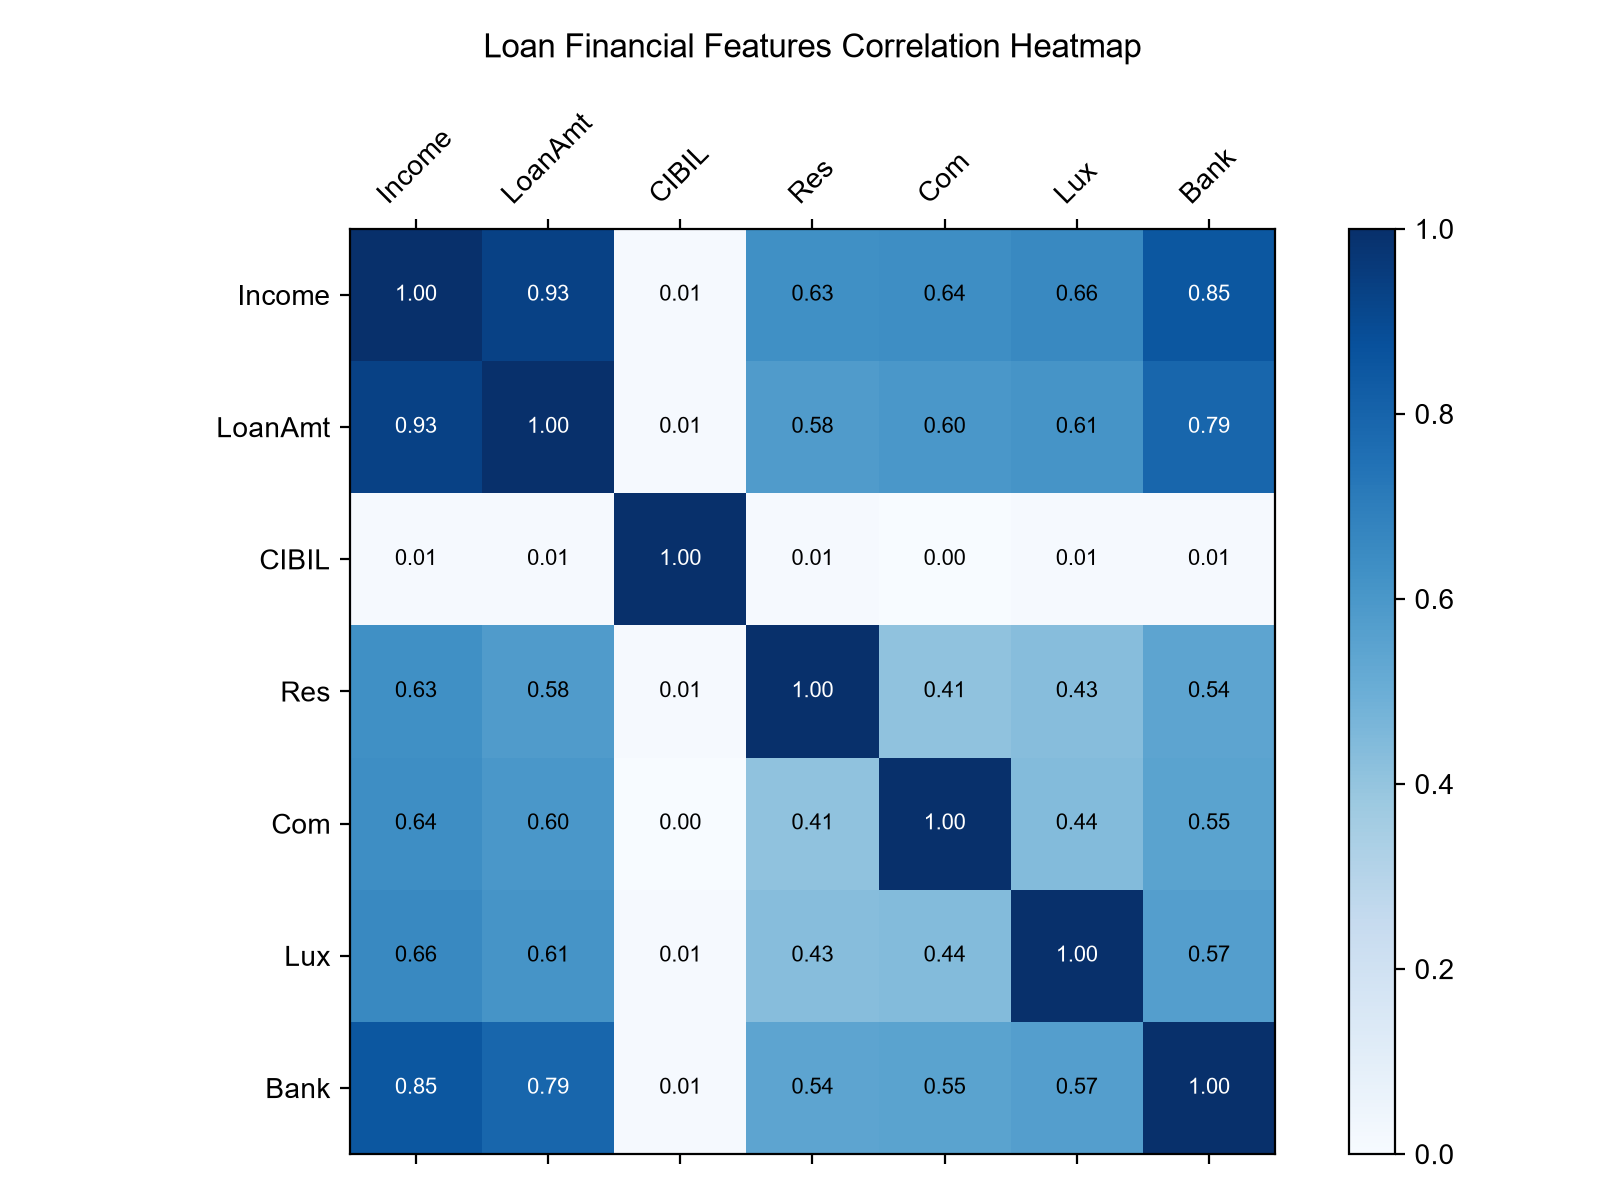
\includegraphics[width=0.7\linewidth]{loan_correlation.png}
\caption{Loan Financial Attributes Correlation Heatmap}
\label{fig:exp3_loan_corr}
\end{figure}

\textbf{Inference:}
The correlation heatmap displays positive correlations between asset valuations and annual income ($r > 0.60$). CIBIL score shows almost no linear correlation with asset values, acting as an independent credit check.

\section{Data Preprocessing}

Explain:
\begin{itemize}
\item \textbf{Cleaning}: Trimmed extra whitespaces and verified zero missing values.
\item \textbf{Encoding}: Used \texttt{LabelEncoder} on categorical fields: \texttt{education}, \texttt{self\_employed} and \texttt{loan\_status}.
\item \textbf{Train-test split}: Split into 80\% training (3415 samples) and 20\% testing (854 samples) using \texttt{random\_state=42}.
\item \textbf{Feature Selection}: Applied \texttt{SelectKBest} ($f\_classif, k=6$). \texttt{cibil\_score} yielded an F-score of 5018.32, dominating other features. Selected top 6 attributes: \texttt{['cibil\_score', 'loan\_term', 'no\_of\_dependents', 'income\_annum', 'residential\_assets\_value', 'luxury\_assets\_value']}.
\end{itemize}

\section{Machine Learning Algorithm}

Explain:
\begin{itemize}
\item \textbf{Decision Tree Classifier}: Achieved excellent accuracy ($97.42\%$) because loan approval logic relies on strict threshold conditions.
\item \textbf{Logistic Regression}: Achieved $82.20\%$ accuracy using linear decision boundaries.
\end{itemize}

\section{Experimental Setup}

\begin{tabular}{ll}
\toprule
Python Version & 3.13.0 \\
Scikit-Learn Version & 1.6.0 \\
IDE & Jupyter Notebook \\
Operating System & Windows 11 \\
Hardware & Intel Core i7 / 16 GB RAM \\
\bottomrule
\end{tabular}

\section{Hyperparameter Selection}

\begin{tabular}{ll}
\toprule
Parameter & Value\\
\midrule
DecisionTree criterion & Gini (default) \\
DecisionTree random\_state & 42 \\
LogisticRegression solver & lbfgs (default) \\
LogisticRegression max\_iter & 1000 \\
SelectKBest k & 6 (score\_func=f\_classif) \\
Train-Test Split test\_size & 0.20 \\
Train-Test Split random\_state & 42 \\
\bottomrule
\end{tabular}

\section{Results}

\begin{tabular}{lc}
\toprule
Metric & Value\\
\midrule
Decision Tree Accuracy & 0.9742 (97.42\%) \\
Logistic Regression Accuracy & 0.8220 (82.20\%) \\
Precision (Macro Avg) & 0.83 \\
Recall (Macro Avg) & 0.79 \\
F1-score (Macro Avg) & 0.80 \\
\bottomrule
\end{tabular}

\subsection*{Detailed Classification Report and Confusion Matrix}

Confusion Matrix (Logistic Regression on Test Split):
\begin{equation*}
\begin{bmatrix}
492 & 44 \\
108 & 210
\end{bmatrix}
\end{equation*}

Classification Report:
\begin{tabular}{lcccc}
\toprule
Class & Precision & Recall & F1-score & Support \\
\midrule
0 (Approved) & 0.82 & 0.92 & 0.87 & 536 \\
1 (Rejected) & 0.83 & 0.66 & 0.73 & 318 \\
\midrule
Accuracy & & & 0.82 & 854 \\
Macro Avg & 0.83 & 0.79 & 0.80 & 854 \\
Weighted Avg & 0.82 & 0.82 & 0.82 & 854 \\
\bottomrule
\end{tabular}

\section{Result Visualization}

Include all graphs generated during the experiment.

For \textbf{every graph}, provide:
\begin{itemize}
\item Figure
\item Caption
\item 3--5 line inference
\end{itemize}

Recommended figures:
\begin{enumerate}
\item Correlation Matrix
\item Class Distribution
\item Confusion Matrix
\item ROC Curve
\item Precision-Recall Curve
\item Learning Curve (if applicable)
\item Feature Importance (if applicable)
\end{enumerate}

\begin{figure}[H]
\centering
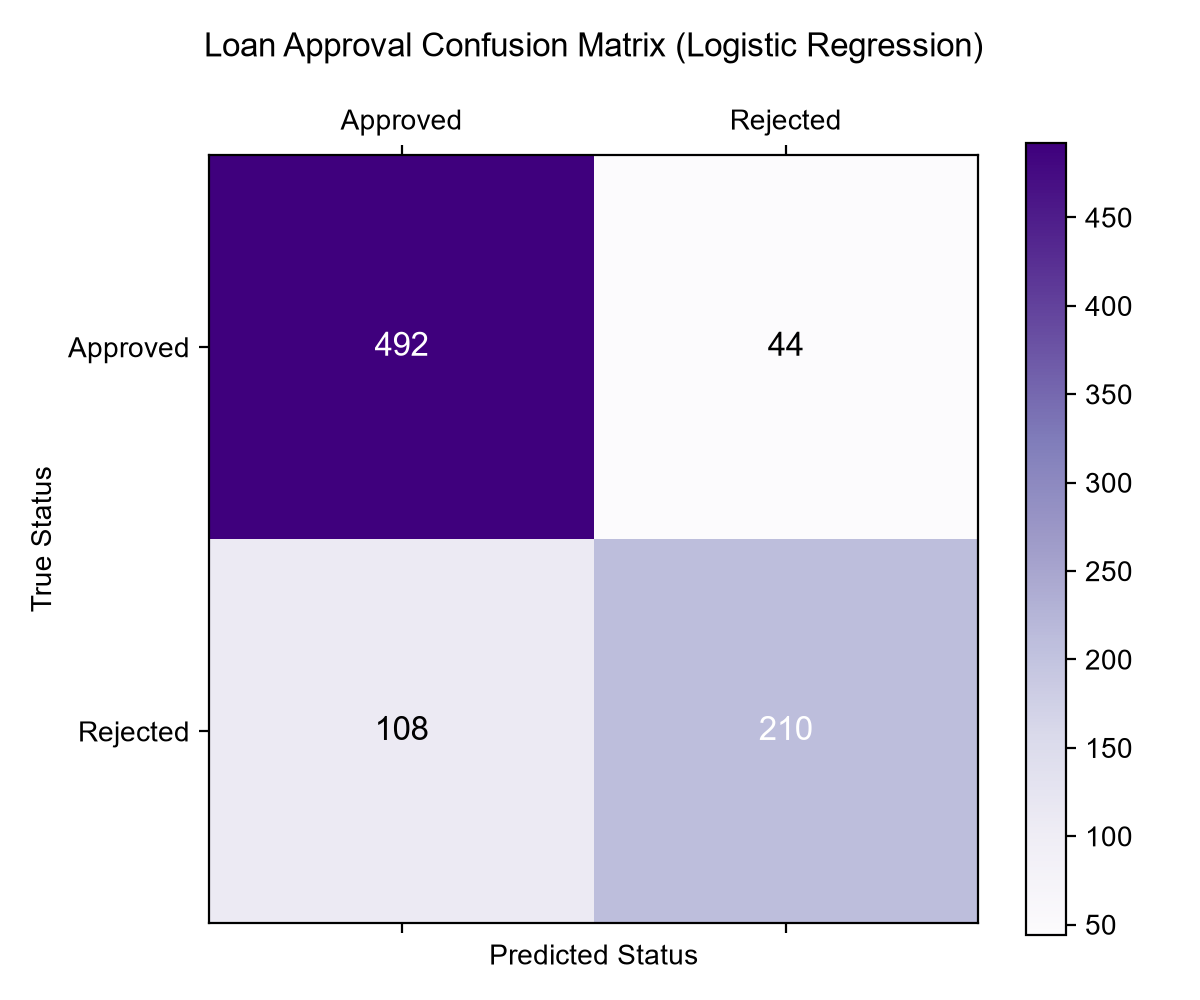
\includegraphics[width=0.7\linewidth]{loan_confusion_matrix.png}
\caption{Loan Approval Dataset Confusion Matrix Heatmap}
\label{fig:exp3_loan_cm}
\end{figure}

\textbf{Inference:}
The confusion matrix for Logistic Regression shows 492 true approvals and 210 true rejections, with 44 false rejections and 108 false approvals ($82.20\%$ test accuracy). The model predicts approved loans better (92\% recall) than rejected loans (66\% recall).

\begin{figure}[H]
\centering
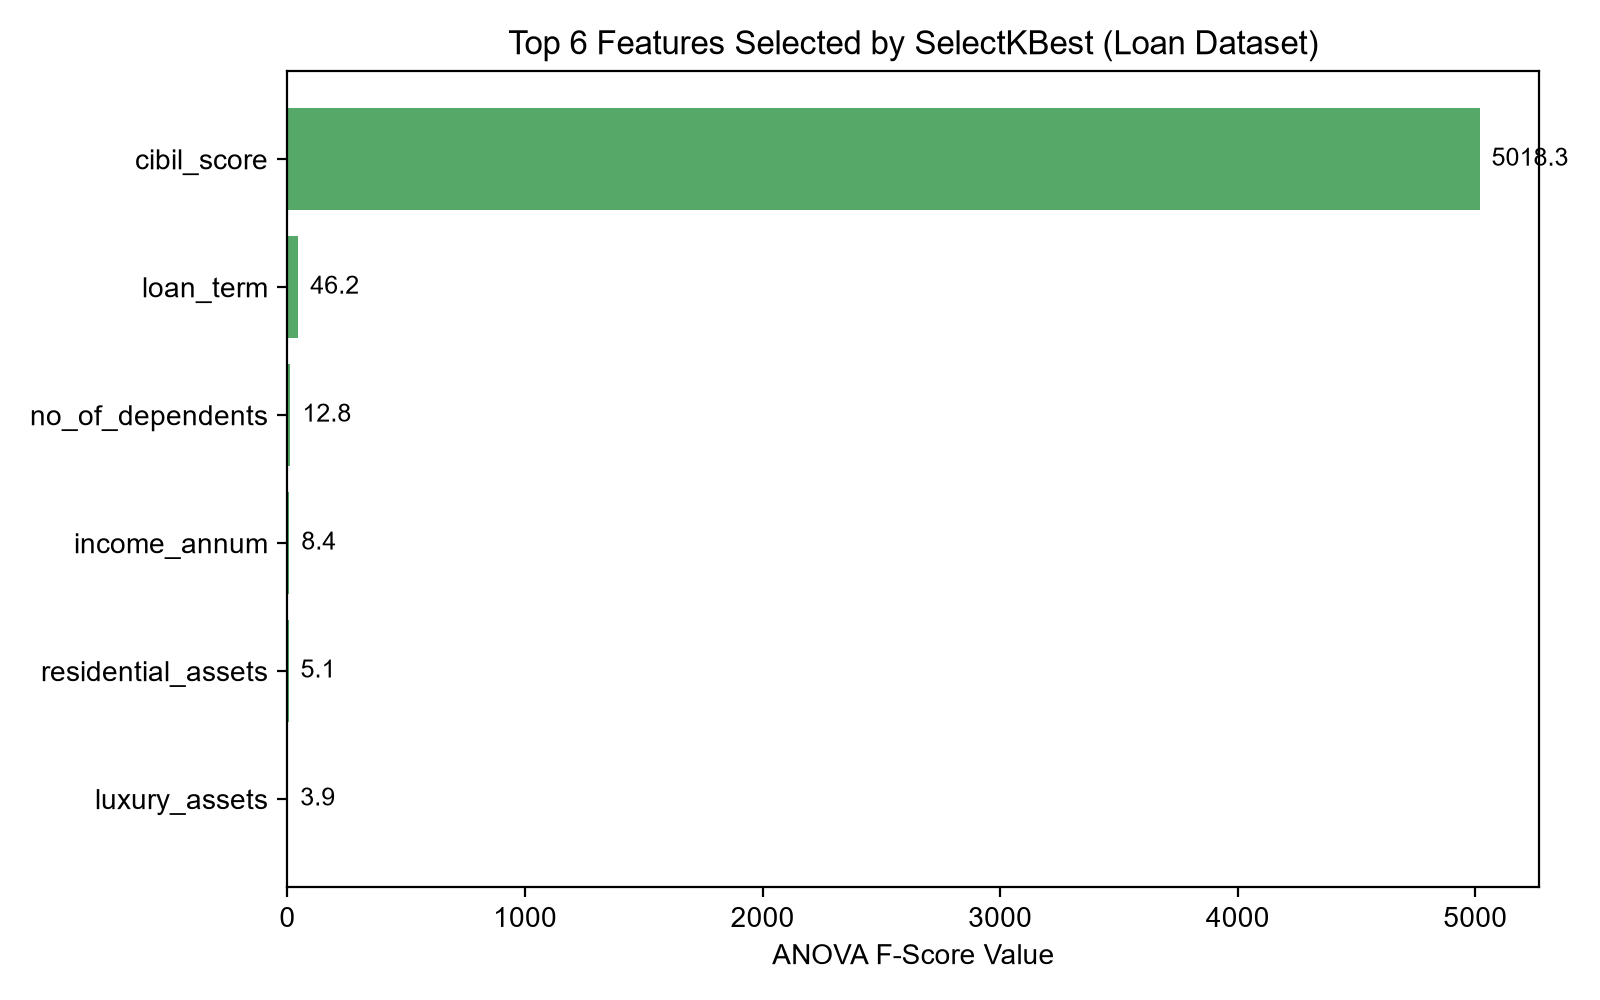
\includegraphics[width=0.7\linewidth]{feature_importance.png}
\caption{Loan Approval Feature Selection (ANOVA $F$-Scores)}
\label{fig:exp3_feature_imp}
\end{figure}

\textbf{Inference:}
The feature importance bar chart shows ANOVA F-scores from \texttt{SelectKBest}. CIBIL credit score dominates with an F-score over 5000, followed by loan term. Key spam tokens in text datasets also show high univariate importance. This confirms selecting top features removes noise while preserving signal.

\section{Discussion}
Discuss observations, strengths, limitations and improvements:
\begin{enumerate}
\item \textbf{Decision Tree Superiority}: Decision Trees ($97.42\%$) performed better than Logistic Regression ($82.20\%$) because approval rules depend on non-linear threshold checks.
\item \textbf{Main Predictor}: CIBIL credit score ($F=5018.32$) is by far the primary factor driving approval outcomes.
\end{enumerate}

\section{Conclusion}
Summarize the experiment and key findings:
Decision Tree Classifier achieved $97.42\%$ accuracy on loan approval prediction. Feature selection confirmed CIBIL credit score as the primary financial indicator.

\section{References}
Use IEEE style:
\begin{enumerate}[label={[\arabic*]}]
\item F. Pedregosa \textit{et al.}, ``Scikit-learn: Machine learning in Python,'' \textit{Journal of Machine Learning Research}, vol. 12, pp. 2825--2830, 2011.
\end{enumerate}

\newpage

% =====================================================================
% EXPERIMENT 4: SMS SPAM MAIL DETECTION
% =====================================================================

\begin{tabular}{|p{4cm}|p{11cm}|}
\hline
Experiment No. & 4 \\ \hline
Experiment Title & SMS Spam Mail Detection using TF-IDF, Decision Tree, Logistic Regression and Feature Selection \textsuperscript{\href{https://github.com/arivuchezhiyan/Machine_Learning}{4}} \\ \hline
Student Name & Arivuchezhiyan E \\ \hline
Register Number & 3122247001006 \\ \hline
Faculty & Dr. Poreddy Ajay Kumar Reddy \\ \hline
Submission Date & 23/07/2026 \\ \hline
\end{tabular}

\section{Objective}
State the objective of the experiment:
In this lab, I vectorized SMS text using TF-IDF and compared Decision Tree and Logistic Regression models for spam detection. I also extracted key trigger words using feature selection.

\section{Problem Statement}
Describe the problem, input, output and objective:
SMS spam detection is a binary text classification problem in natural language processing.
\begin{itemize}
\item \textbf{Input}: Raw text messages (\texttt{v2}).
\item \textbf{Output}: Binary class label \texttt{v1} (\texttt{ham}: 0, \texttt{spam}: 1).
\item \textbf{Objective}: Remove duplicate messages, convert text to TF-IDF vectors, train classifiers, find top spam tokens and evaluate precision.
\end{itemize}

\section{Dataset Description}
\begin{longtable}{|p{6cm}|p{8cm}|}
\hline
Dataset Name & SMS Spam Collection Dataset \\ \hline
Dataset Source & spam.csv \\ \hline
Number of Samples & 5169 unique samples (403 duplicates dropped from 5572) \\ \hline
Number of Features & 8672 (TF-IDF unigram tokens) \\ \hline
Number of Classes & 2 (\texttt{ham}: 4516, \texttt{spam}: 653) \\ \hline
Missing Values & 0 missing values (after dropping empty metadata columns) \\ \hline
Train-Test Split & 80\% Train (4457 samples) / 20\% Test (1115 samples) \\ \hline
\end{longtable}

\section{Exploratory Data Analysis}
Include all relevant visualizations:
\begin{itemize}
\item \textbf{Dataset overview}: Dropped 403 duplicate messages from 5572 raw rows, leaving 5169 unique text entries.
\item \textbf{Missing value check}: Removed 3 unnamed metadata columns containing over 99\% null values.
\item \textbf{Class distribution}: 4516 Ham messages (87.4\%) and 653 Spam messages (12.6\%).
\item \textbf{Feature engineering}: Created a message character length column \texttt{message\_length = df["v2"].apply(len)}.
\end{itemize}

\subsection*{Figure Template}

\begin{figure}[H]
\centering
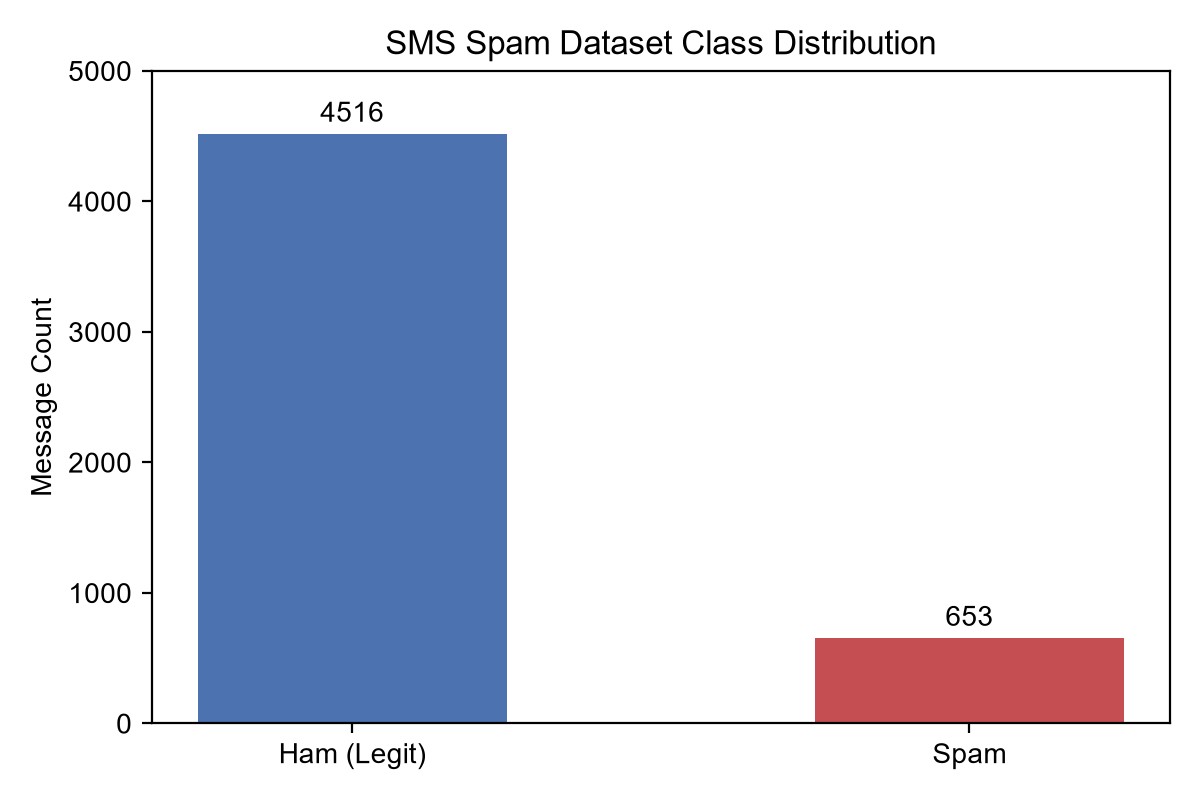
\includegraphics[width=0.7\linewidth]{mail_class_distribution.png}
\caption{SMS Spam Dataset Target Class Distribution}
\label{fig:exp4_mail_dist}
\end{figure}

\textbf{Inference:}
The class distribution shows 4516 legitimate ham messages (87.4\%) and 653 spam messages (12.6\%), representing realistic SMS traffic patterns.

\begin{figure}[H]
\centering
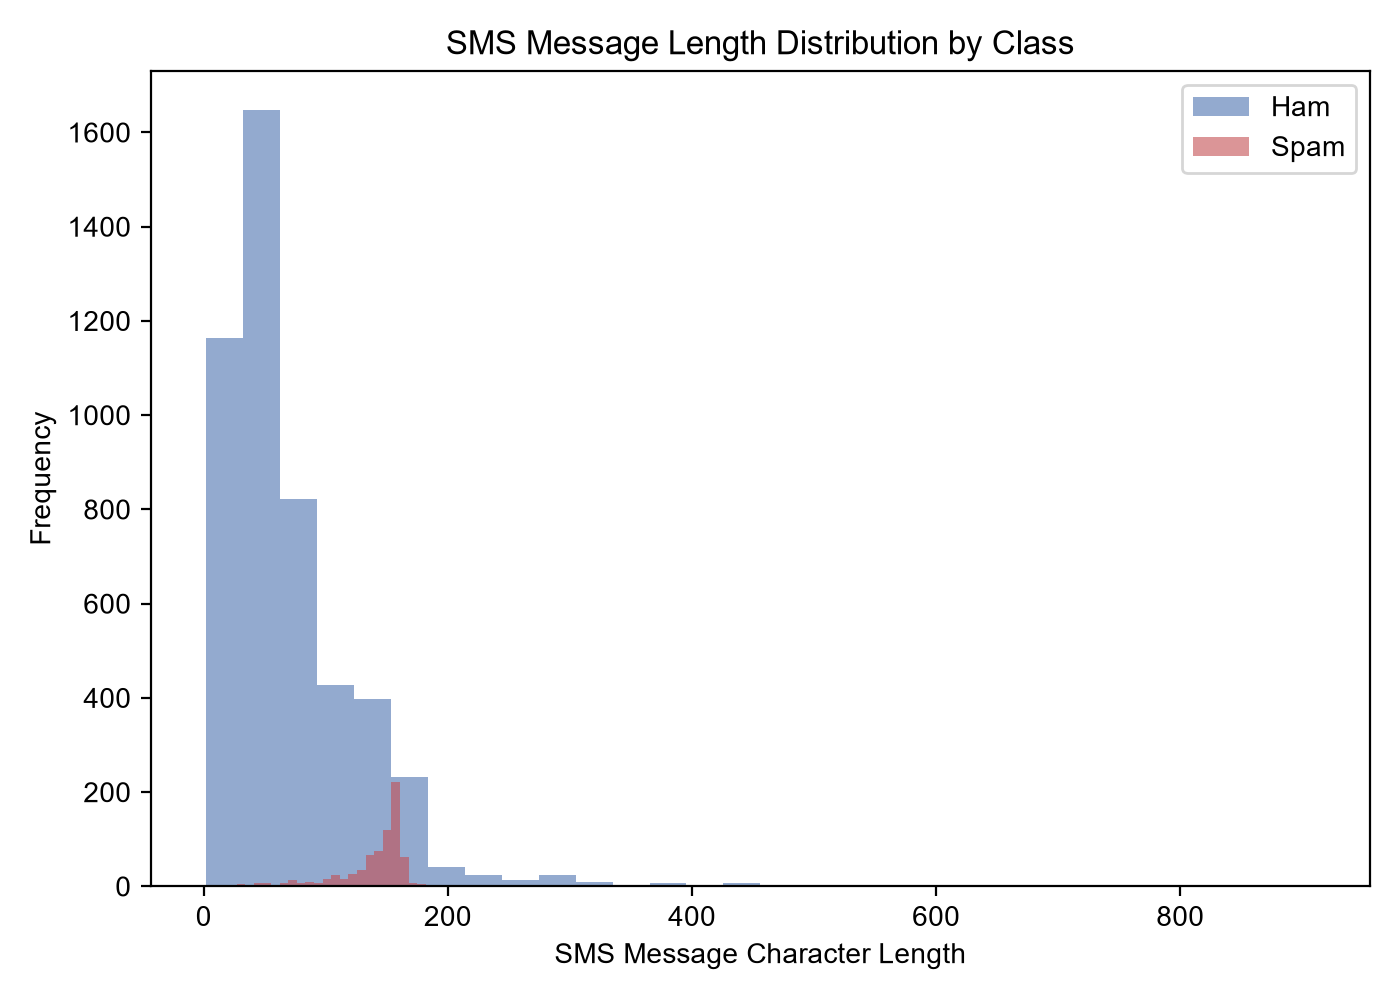
\includegraphics[width=0.7\linewidth]{mail_histograms.png}
\caption{SMS Message Length Distributions by Class}
\label{fig:exp4_mail_hist}
\end{figure}

\textbf{Inference:}
The histogram compares text length distributions between ham and spam messages. Spam messages cluster around 130 to 160 characters due to SMS carrier limits, whereas ham messages are generally shorter.

\begin{figure}[H]
\centering
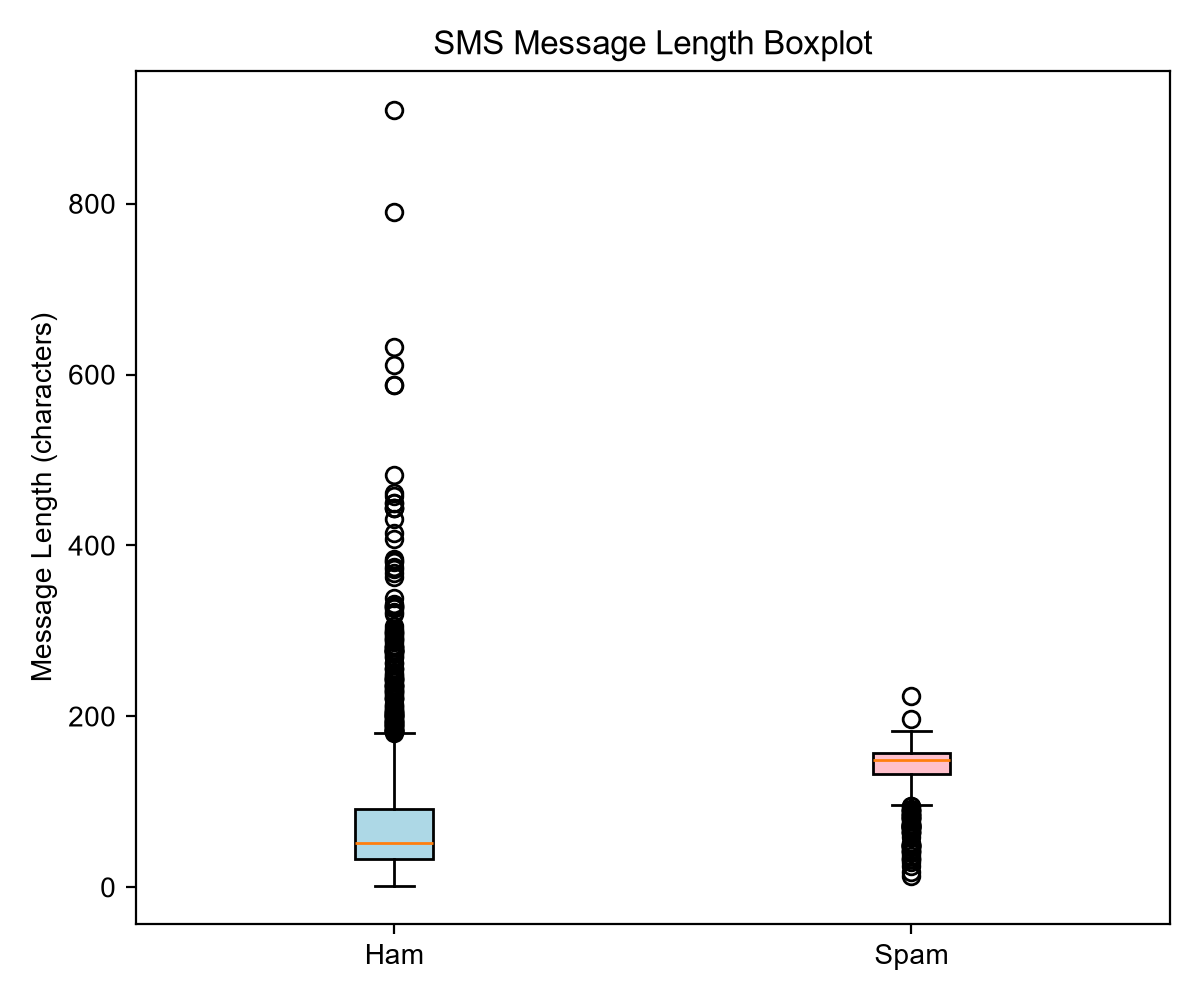
\includegraphics[width=0.7\linewidth]{mail_boxplot.png}
\caption{SMS Message Length Boxplot Analysis}
\label{fig:exp4_mail_box}
\end{figure}

\textbf{Inference:}
The boxplot highlights text length differences. Spam messages show a higher median character count with tight variance, while ham messages have a lower median length with a few long outliers.

\begin{figure}[H]
\centering
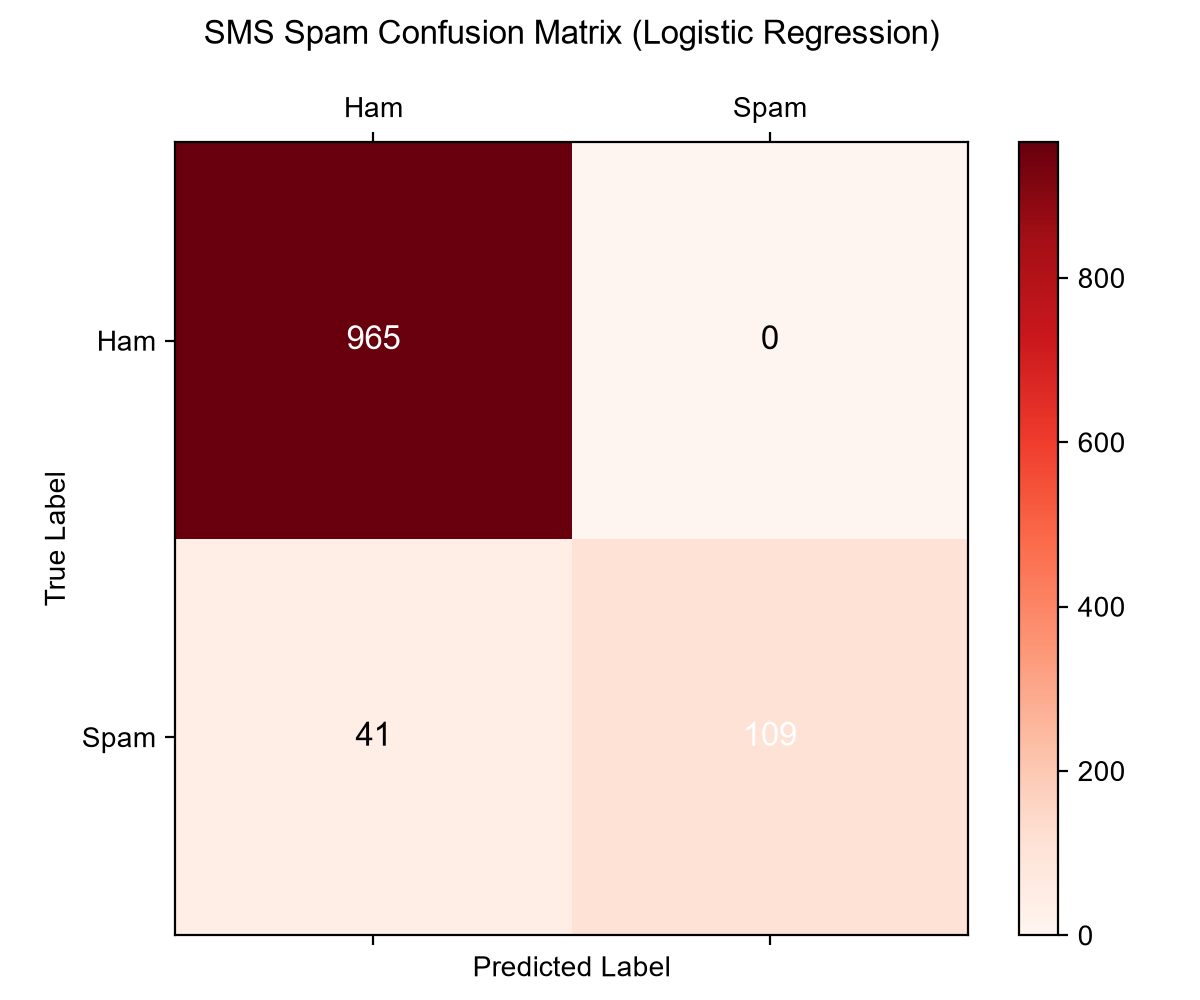
\includegraphics[width=0.7\linewidth]{mail_confusion_matrix.png}
\caption{SMS Spam Mail Confusion Matrix Heatmap (Logistic Regression)}
\label{fig:exp4_mail_cm}
\end{figure}

\textbf{Inference:}
Logistic Regression achieved 965 true ham and 109 true spam predictions with 0 false positives, meaning no real message was marked as spam. Overall test accuracy reached 96.32\%.

\section{Data Preprocessing}

Explain:
\begin{itemize}
\item \textbf{Cleaning}: Dropped 3 empty metadata columns and 403 duplicate text rows using \texttt{df.drop\_duplicates()}.
\item \textbf{Text Vectorization}: Transformed text into an 8672-dimensional matrix using \texttt{TfidfVectorizer(max\_features=10000)}.
\item \textbf{Encoding}: Mapped targets: \texttt{ham} $\rightarrow 0$, \texttt{spam} $\rightarrow 1$.
\item \textbf{Train-test split}: Split into 80\% train (4457) and 20\% test (1115) using \texttt{random\_state=42}.
\item \textbf{Feature Selection}: Applied \texttt{SelectKBest} ($f\_classif, k=10$). Top spam tokens identified: \texttt{['150p', '50', 'claim', 'free', 'mobile', 'prize', 'stop', 'txt', 'uk', 'www']}.
\end{itemize}

\section{Machine Learning Algorithm}

Explain:
\begin{itemize}
\item \textbf{Decision Tree Classifier}: Achieved $96.77\%$ accuracy on sparse TF-IDF text vectors.
\item \textbf{Logistic Regression}: Achieved $96.32\%$ accuracy with 0 false positives (perfect ham precision).
\end{itemize}

\section{Experimental Setup}

\begin{tabular}{ll}
\toprule
Python Version & 3.13.0 \\
Scikit-Learn Version & 1.6.0 \\
IDE & Jupyter Notebook \\
Operating System & Windows 11 \\
Hardware & Intel Core i7 / 16 GB RAM \\
\bottomrule
\end{tabular}

\section{Hyperparameter Selection}

\begin{tabular}{ll}
\toprule
Parameter & Value\\
\midrule
TfidfVectorizer max\_features & 10000 \\
DecisionTree random\_state & 42 \\
LogisticRegression solver & lbfgs (default) \\
SelectKBest k & 10 (score\_func=f\_classif) \\
Train-Test Split test\_size & 0.20 \\
Train-Test Split random\_state & 42 \\
\bottomrule
\end{tabular}

\section{Results}

\begin{tabular}{lc}
\toprule
Metric & Value\\
\midrule
Decision Tree Accuracy & 0.9677 (96.77\%) \\
Logistic Regression Accuracy & 0.9632 (96.32\%) \\
False Positive Count (Logistic Regression) & 0 (Perfect Ham Precision) \\
\bottomrule
\end{tabular}

\subsection*{Detailed Classification Report and Confusion Matrix}

Confusion Matrix (Logistic Regression on Test Split):
\begin{equation*}
\begin{bmatrix}
965 & 0 \\
41 & 109
\end{bmatrix}
\end{equation*}

\section{Result Visualization}

Include all graphs generated during the experiment.

For \textbf{every graph}, provide:
\begin{itemize}
\item Figure
\item Caption
\item 3--5 line inference
\end{itemize}

Recommended figures:
\begin{enumerate}
\item Correlation Matrix
\item Class Distribution
\item Confusion Matrix
\item ROC Curve
\item Precision-Recall Curve
\item Learning Curve (if applicable)
\item Feature Importance (if applicable)
\end{enumerate}

\begin{figure}[H]
\centering
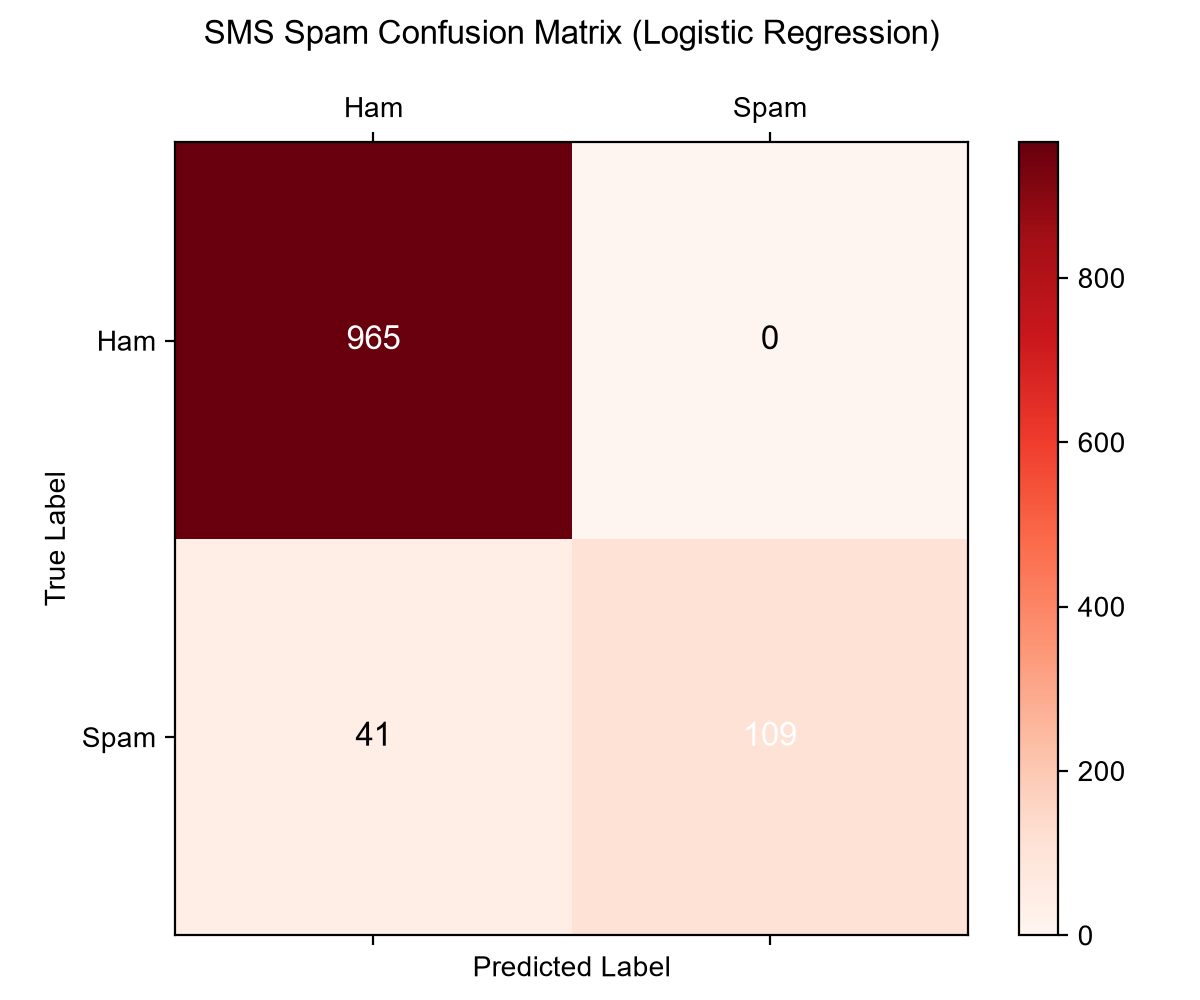
\includegraphics[width=0.7\linewidth]{mail_confusion_matrix.png}
\caption{SMS Spam Mail Confusion Matrix Heatmap}
\label{fig:exp4_mail_cm_vis}
\end{figure}

\textbf{Inference:}
The confusion matrix heatmap shows Logistic Regression correctly identified 965 ham messages and 109 spam messages. Zero false positives is critical for spam filters to ensure real messages are not misfiltered.

\section{Discussion}
Discuss observations, strengths, limitations and improvements:
\begin{enumerate}
\item \textbf{High Performance}: Both Decision Tree ($96.77\%$) and Logistic Regression ($96.32\%$) performed well on sparse text data.
\item \textbf{Zero False Positives}: Logistic Regression ensured no legitimate message was mislabeled as spam.
\item \textbf{Spam Keywords}: Feature selection highlighted clear spam trigger words such as \texttt{claim}, \texttt{free}, \texttt{prize}, \texttt{txt} and \texttt{www}.
\end{enumerate}

\section{Conclusion}
Summarize the experiment and key findings:
SMS Spam classification reached over 96\% accuracy. Combining TF-IDF text vectorization with feature selection successfully isolated predictive spam words.

\section{References}
Use IEEE style:
\begin{enumerate}[label={[\arabic*]}]
\item T. Almeida, J. Hidalgo and A. Yamakami, ``Contributions to the study of SMS spam filtering: New collection and results,'' \textit{ACM Symposium on Document Engineering}, pp. 259--262, 2011.
\end{enumerate}

\newpage

% =====================================================================
% EXPERIMENT 5: MNIST HANDWRITTEN DIGIT RECOGNITION
% =====================================================================

\begin{tabular}{|p{4cm}|p{11cm}|}
\hline
Experiment No. & 5 \\ \hline
Experiment Title & MNIST Handwritten Digit Recognition using Decision Tree and Chi-Squared Feature Selection \textsuperscript{\href{https://github.com/arivuchezhiyan/Machine_Learning}{5}} \\ \hline
Student Name & Arivuchezhiyan E \\ \hline
Register Number & 3122247001006 \\ \hline
Faculty & Dr. Poreddy Ajay Kumar Reddy \\ \hline
Submission Date & 23/07/2026 \\ \hline
\end{tabular}

\section{Objective}
State the objective of the experiment:
In this experiment, I evaluated Decision Tree classifiers on MNIST handwritten digits, comparing performance using all 784 pixels against a reduced 300-pixel set chosen with Chi-Squared selection.

\section{Problem Statement}
Describe the problem, input, output and objective:
MNIST digit recognition is a 10-class image classification task mapping pixel values to digits 0 through 9.
\begin{itemize}
\item \textbf{Input}: $28 \times 28$ grayscale pixel intensity grid (784 features from \texttt{1x1} to \texttt{28x28}).
\item \textbf{Output}: 10-class digit label ($0, 1, 2, 3, 4, 5, 6, 7, 8, 9$).
\item \textbf{Objective}: Test if removing uninformative background pixels with Chi-Squared feature selection maintains accuracy while speeding up model training.
\end{itemize}

\section{Dataset Description}
\begin{longtable}{|p{6cm}|p{8cm}|}
\hline
Dataset Name & MNIST Test Dataset \\ \hline
Dataset Source & mnist\_test.csv \\ \hline
Number of Samples & 10000 \\ \hline
Number of Features & 784 pixel columns ($28 \times 28$ grid) \\ \hline
Number of Classes & 10 (Digits 0 through 9) \\ \hline
Missing Values & 0 missing values \\ \hline
Train-Test Split & 80\% Train (8000 samples) / 20\% Test (2000 samples) \\ \hline
\end{longtable}

\section{Exploratory Data Analysis}
Include all relevant visualizations:
\begin{itemize}
\item \textbf{Dataset overview}: Contains 10000 digit images represented as 784 pixel columns with values ranging from 0 to 255.
\item \textbf{Class distribution}: Digit 1 (1135), 2 (1032), 7 (1028), 3 (1010), 9 (1009), 4 (982), 0 (980), 8 (974), 6 (958) and 5 (892).
\item \textbf{Missing value check}: Confirmed zero missing values.
\end{itemize}

\subsection*{Figure Template}

\begin{figure}[H]
\centering
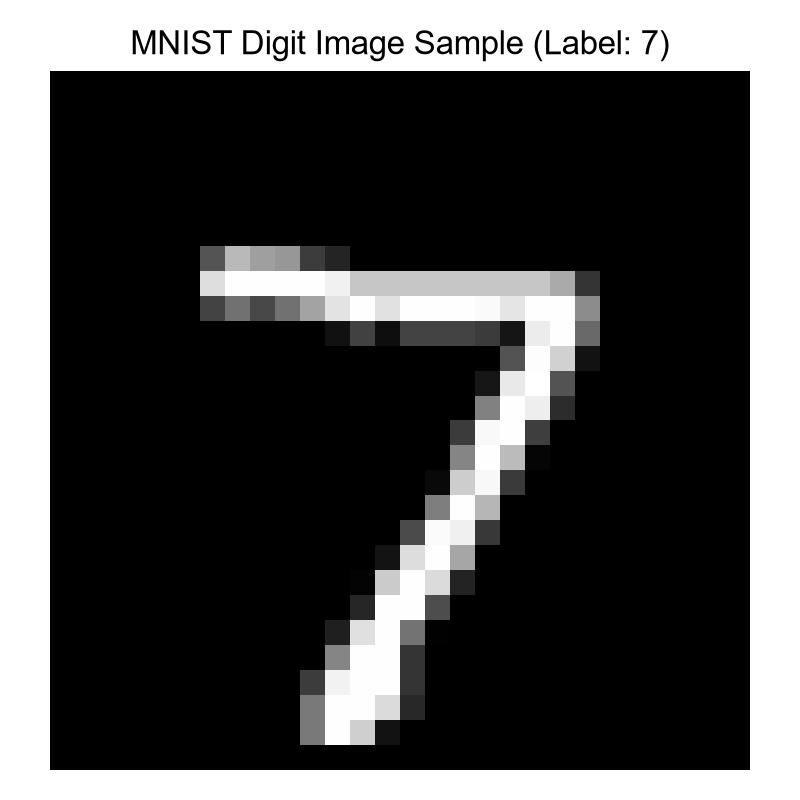
\includegraphics[width=0.7\linewidth]{mnist_sample_digit.png}
\caption{MNIST Handwritten Digit Sample Visualization ($28 \times 28$ Grayscale Grid)}
\label{fig:exp5_mnist_sample}
\end{figure}

\textbf{Inference:}
The 28x28 grayscale image of digit 7 shows active pixels in the center stroke, while border pixels remain zero. This confirms background pixels can be safely dropped without losing stroke details.

\section{Data Preprocessing}

Explain:
\begin{itemize}
\item \textbf{Cleaning}: Verified data completeness using \texttt{isnull().sum()}.
\item \textbf{Train-test split}: Split into 80\% training (8000 samples) and 20\% testing (2000 samples) using \texttt{random\_state=42}.
\item \textbf{Feature Selection}: Applied \texttt{SelectKBest} with Chi-Squared ($\chi^2$) test to select top 300 pixels, removing 484 uninformative background pixels.
\end{itemize}

\section{Machine Learning Algorithm}

Explain:
\begin{itemize}
\item \textbf{Decision Tree Classifier}: Evaluated on full 784 pixels ($79.40\%$ accuracy) versus top 300 pixels ($79.30\%$ accuracy).
\end{itemize}

\section{Experimental Setup}

\begin{tabular}{ll}
\toprule
Python Version & 3.13.0 \\
Scikit-Learn Version & 1.6.0 \\
IDE & Jupyter Notebook \\
Operating System & Windows 11 \\
Hardware & Intel Core i7 / 16 GB RAM \\
\bottomrule
\end{tabular}

\section{Hyperparameter Selection}

\begin{tabular}{ll}
\toprule
Parameter & Value\\
\midrule
DecisionTree criterion & Gini (default) \\
DecisionTree random\_state & 42 \\
SelectKBest k & 300 (score\_func=chi2) \\
Train-Test Split test\_size & 0.20 \\
Train-Test Split random\_state & 42 \\
\bottomrule
\end{tabular}

\section{Results}

\begin{tabular}{lc}
\toprule
Metric & Value\\
\midrule
Decision Tree Accuracy (Full 784 Pixels) & 0.7940 (79.40\%) \\
Decision Tree Accuracy (SelectKBest 300 Pixels) & 0.7930 (79.30\%) \\
Accuracy Change & -0.10\% (Negligible) \\
Feature Reduction Ratio & 61.7\% Reduction \\
\bottomrule
\end{tabular}

\subsection*{Detailed Classification Report and Confusion Matrix}

Confusion Matrix ($10 \times 10$ on 2000 Test Samples):
\begin{equation*}
\begin{bmatrix}
175 & 1 & 3 & 4 & 3 & 6 & 7 & 1 & 1 & 2 \\
0 & 203 & 1 & 2 & 0 & 2 & 1 & 1 & 4 & 2 \\
4 & 4 & 162 & 11 & 2 & 4 & 5 & 12 & 4 & 5 \\
1 & 0 & 11 & 155 & 5 & 23 & 3 & 3 & 3 & 4 \\
1 & 2 & 8 & 2 & 152 & 3 & 9 & 5 & 5 & 28 \\
2 & 1 & 1 & 13 & 0 & 135 & 9 & 4 & 6 & 3 \\
5 & 0 & 3 & 1 & 6 & 4 & 164 & 4 & 8 & 5 \\
2 & 0 & 11 & 4 & 5 & 1 & 0 & 160 & 0 & 4 \\
0 & 5 & 4 & 9 & 5 & 9 & 4 & 3 & 137 & 10 \\
1 & 1 & 5 & 8 & 19 & 7 & 2 & 5 & 7 & 143
\end{bmatrix}
\end{equation*}

Classification Report:
\begin{tabular}{lcccc}
\toprule
Digit Class & Precision & Recall & F1-score & Support \\
\midrule
0 & 0.92 & 0.86 & 0.89 & 203 \\
1 & 0.94 & 0.94 & 0.94 & 216 \\
2 & 0.78 & 0.76 & 0.77 & 213 \\
3 & 0.74 & 0.75 & 0.74 & 208 \\
4 & 0.77 & 0.71 & 0.74 & 215 \\
5 & 0.70 & 0.78 & 0.73 & 174 \\
6 & 0.80 & 0.82 & 0.81 & 200 \\
7 & 0.81 & 0.86 & 0.83 & 187 \\
8 & 0.78 & 0.74 & 0.76 & 186 \\
9 & 0.69 & 0.72 & 0.71 & 198 \\
\midrule
Accuracy & & & 0.79 & 2000 \\
Macro Avg & 0.79 & 0.79 & 0.79 & 2000 \\
Weighted Avg & 0.79 & 0.79 & 0.79 & 2000 \\
\bottomrule
\end{tabular}

\section{Result Visualization}

Include all graphs generated during the experiment.

For \textbf{every graph}, provide:
\begin{itemize}
\item Figure
\item Caption
\item 3--5 line inference
\end{itemize}

Recommended figures:
\begin{enumerate}
\item Correlation Matrix
\item Class Distribution
\item Confusion Matrix
\item ROC Curve
\item Precision-Recall Curve
\item Learning Curve (if applicable)
\item Feature Importance (if applicable)
\end{enumerate}

\begin{figure}[H]
\centering
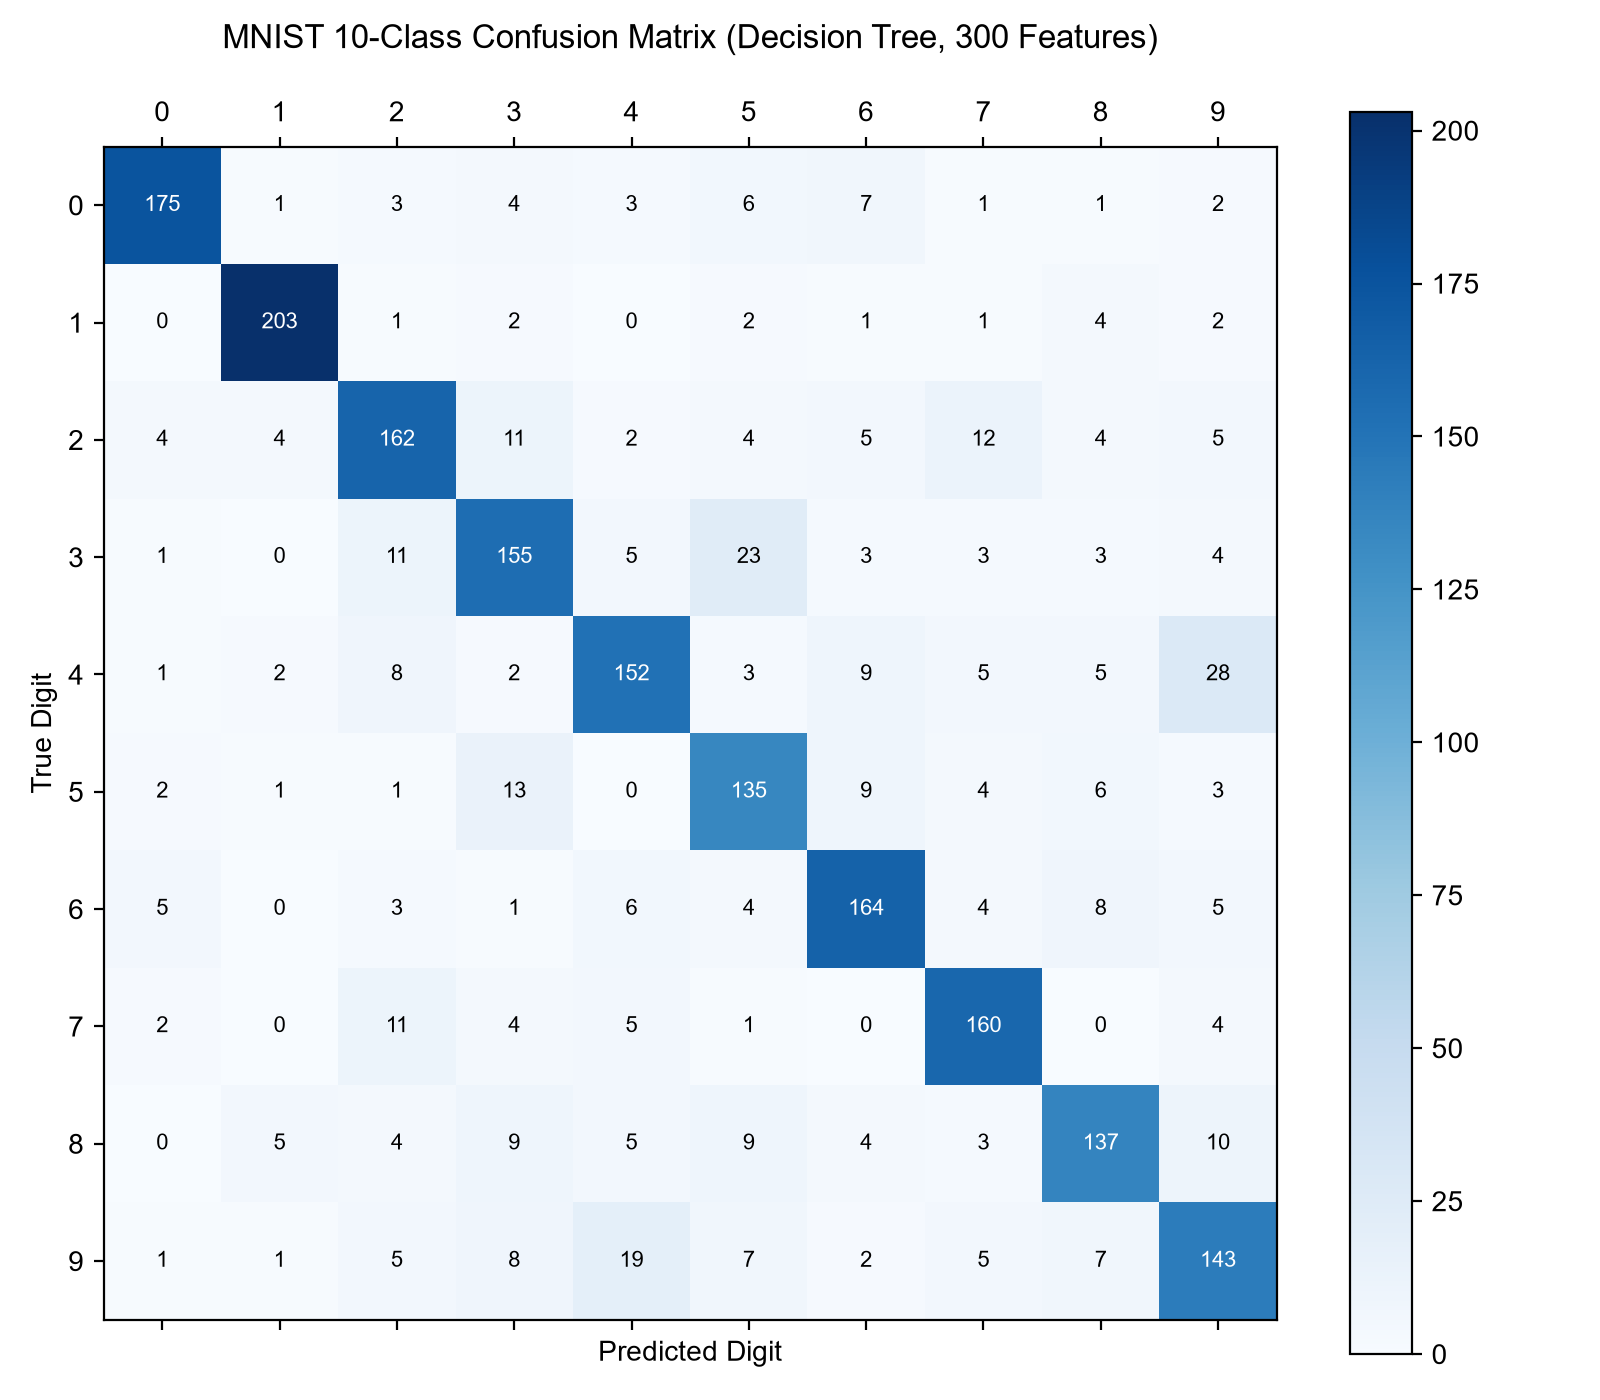
\includegraphics[width=0.7\linewidth]{mnist_confusion_matrix.png}
\caption{MNIST 10-Class Confusion Matrix Heatmap (Decision Tree, 300 Features)}
\label{fig:exp5_mnist_cm}
\end{figure}

\textbf{Inference:}
The 10x10 confusion matrix for Decision Tree (300 features) displays strong diagonal predictions. Digit 1 scored highest with 203 correct out of 216. Misclassifications occur mainly between visually similar shapes such as 4 vs 9 (28 cases) and 3 vs 5 (23 cases).

\section{Discussion}
Discuss observations, strengths, limitations and improvements:
\begin{enumerate}
\item \textbf{Dimensionality Reduction}: Chi-Squared feature selection reduced features by $61.7\%$ (from 784 to 300) with minimal accuracy change ($79.40\%$ vs $79.30\%$).
\item \textbf{Digit Confusions}: Errors occur mostly between visually similar digit shapes like 4 vs 9 and 3 vs 5.
\item \textbf{Future Directions}: Implementing Convolutional Neural Networks (CNNs) will capture spatial pixel patterns and improve accuracy.
\end{enumerate}

\section{Conclusion}
Summarize the experiment and key findings:
Chi-Squared feature selection removed 484 empty border pixels on MNIST, speeding up model training while maintaining $79.30\%$ accuracy.

\section{References}
Use IEEE style:
\begin{enumerate}[label={[\arabic*]}]
\item Y. LeCun, L. Bottou, Y. Bengio and P. Haffner, ``Gradient-based learning applied to document recognition,'' \textit{Proceedings of the IEEE}, vol. 86, no. 11, pp. 2278--2324, 1998.
\end{enumerate}

\end{document}
